\documentclass[chaparabic,ceng,ms,12pt,oneandhalf]{metu}
\usepackage{appendix}
\usepackage{longtable}
\usepackage[pdftex]{hyperref}
\usepackage[all]{hypcap}
\usepackage{todonotes}
\usepackage{graphicx}
\usepackage{caption}
\usepackage{subcaption}
\graphicspath{ {./images/} }
\usepackage{rotating}
\usepackage{xy} 
\usepackage{booktabs}
\usepackage{pifont}
\usepackage{color}
\usepackage{listings}
\usepackage{pdfpages}
\usepackage{array}
\usepackage{algorithm}
\usepackage{algorithmic}
\usepackage{float}
\usepackage{caption}
\usepackage{lastpage}
\usepackage{afterpage}
\usepackage{lipsum}
\usepackage{adjustbox}
\captionsetup{belowskip=12pt,aboveskip=8pt}
\newcommand{\tab}{\hspace*{2em}}
\graphicspath{{Figures/}}
\DeclareGraphicsExtensions{.pdf,.png,.jpg}

% End of Latex Packages

% End of personal stuff
%
% Personal Information 
% ----------------------------
%
% Please check this part and fill in information about your thesis
%
% Name and Surname
\author{Erencan Duymaz}
% Thesis Title English and Turkish
\title{Interleaved Inertial Support of Wind Turbines}
\turkishtitle{Başlık}

\date{June 2018}
 
% prof : Prof. Dr.
% assocprof : Assoc. Prof. Dr.
% assistprof : Assist. Prof. Dr.
% dr : Dr.
%
% Director of Institute
\director[prof]{Gülbin Dural Ünver}
% Head of Department
\headofdept[prof]{Bölüm Başkanı}
%
% Supervisor : English and Turkish
\supervisor[Ass.Prof.Dr.]{Ozan KEYSAN}
% \turkishsupervisor{  } %if you will hard-code the academic title
%
% Affiliation of Supervisor in English and possibly in Turkish
\departmentofsupervisor{Department of Electrical and Electronics Engineering, METU}
%
% Committee Members
% In general members are sorted according to their academic titles
%
% Proffesors (1)
% Associate Professors (2)
% Assistant Professors (3)
% Other (4)
% 
% IMPORTANT:  All affiliatons should fit in a single line
% If affiliation line is broken into two lines you should shorten the affiliation by using 
% abbrevations or any other means
%
% First committee member should be the chair of examining committee
% Typically the chair is one of the highest ranked committee members
% Ask your supervisor if you are not sure
\committeememberi[prof]{Jüri}
\affiliationi{JüriBölüm, METU}
% Second committee member is always your supervisor
\committeememberii[prof]{Jüri}
\affiliationii{JüriBölüm, METU}
% If you are an M.Sc. student and your Co-Supervisor is in your 
% examination committee, then third committee member is always your co-supervisor
%
% IMPORTANT: If you are Ph.D. student your co-supervisor can not be in your 
% examination committee.
\committeememberiii[prof]{Jüri}
\affiliationiii{JüriBölüm, METU}
% Fourth committee member
\committeememberiv[assocprof]{Jüri}
\affiliationiv{JüriBölüm, METU}
% Fifth committee member
\committeememberv[assistprof]{Jüri}
\affiliationv{JüriBölüm, Ankara University}
%
% Keywords : English & Turkish, Comma seperated
\keywords{Keyword1, Keyword2...}
\anahtarklm{AnahtarKelime1, AnahtarKelime2...}
%
% Abstract in English
%
\abstract{Abstract}
%
% Turkish Abstract
%
\oz{Özet Türkçe} 
%
% Dedication 
\dedication{\textit{İthafen...}}
%
%
% Acknowledgements   
\acknowledgments{Teşekkür edilecekler}
%
% End of Personal and Introductory Information
%%%%%%%%%%%%%%%%%%%%%%%%%%%%%%%%%5
\begin{document}
% Preliminaries
\begin{preliminaries}
% If you are willing to use any custom stuff before Chapters, put it here
% Such as List of Abbreviations
% Check the abbreviations.tex for a template list of abbreviations

\begin{glossary}{}

\begin{itemize}[leftmargin=4.5em,align=parleft,labelsep=1cm]
	
\item[AC] 		Alternating Current
\item[AGC] 		Automatic Generation Control
\item[CDF] 		Cumulative Distribution Function
\item[DC] 		Direct Current
\item[DFIG] 	Doubly Fed Induction Generator
\item[EESG] 	Electrically Excited Synchronous Generator
\item[FFR] 		Firm Frequency Response
\item[FSIG] 	Fixed Speed Induction Generator
\item[GSC] 		Grid Side Converter or Controller
\item[HCS] 		Hill-Climb Search
\item[HV]		High Voltage
\item[IGBT] 	Insulated Gate Bipolar Transistor
\item[LSC] 		Line Side Converter or Controller
\item[LVRT] 	Low Voltage Ride-Through
\item[MOSFET] 	Metal Oxide Semiconductor Field Effect Transistor
\item[MSC] 		Machine Side Converter or Controller
\item[PDF] 		Probability Density Function
\item[PI] 		Proportional-integral
\item[PLL] 		Phase-Locked Loop
\item[PMSG] 	Permanent Magnet Synchronous Generator
\item[P\&O] 	Perturb\&Obserb
\item[PSF] 		Power Signal Feedback
\item[RES] 		Renewable Energy System
\item[RoCoF] 	Rate of Change of Frequency

\end{itemize}

\end{glossary}

% End of Preliminaries
\end{preliminaries}
%   
% Latex content Goes Here 
% 
%

\setlength{\parindent}{0em}
\setlength{\parskip}{10pt}


\chapter{INTRODUCTION}
\label{chp:1}
\section{Global Renewable Energy Status}
The share of the renewable energy systems has been reached significant levels. At the end of 2017, the renewable power capacity has reached 2179 GW throughout the world including hydro power plants \cite{InternationalRenewableEnergyAgencyIRENA2018}. Fig. \ref{renewablecap} shows the installed renewable energy capacity for leading countries at the end of 2016 and 2017. China has the biggest installed renewable energy capacity among these countries and increased its capacity by 73 GW in 2017.\par
\begin{figure}[h]
	\centering
	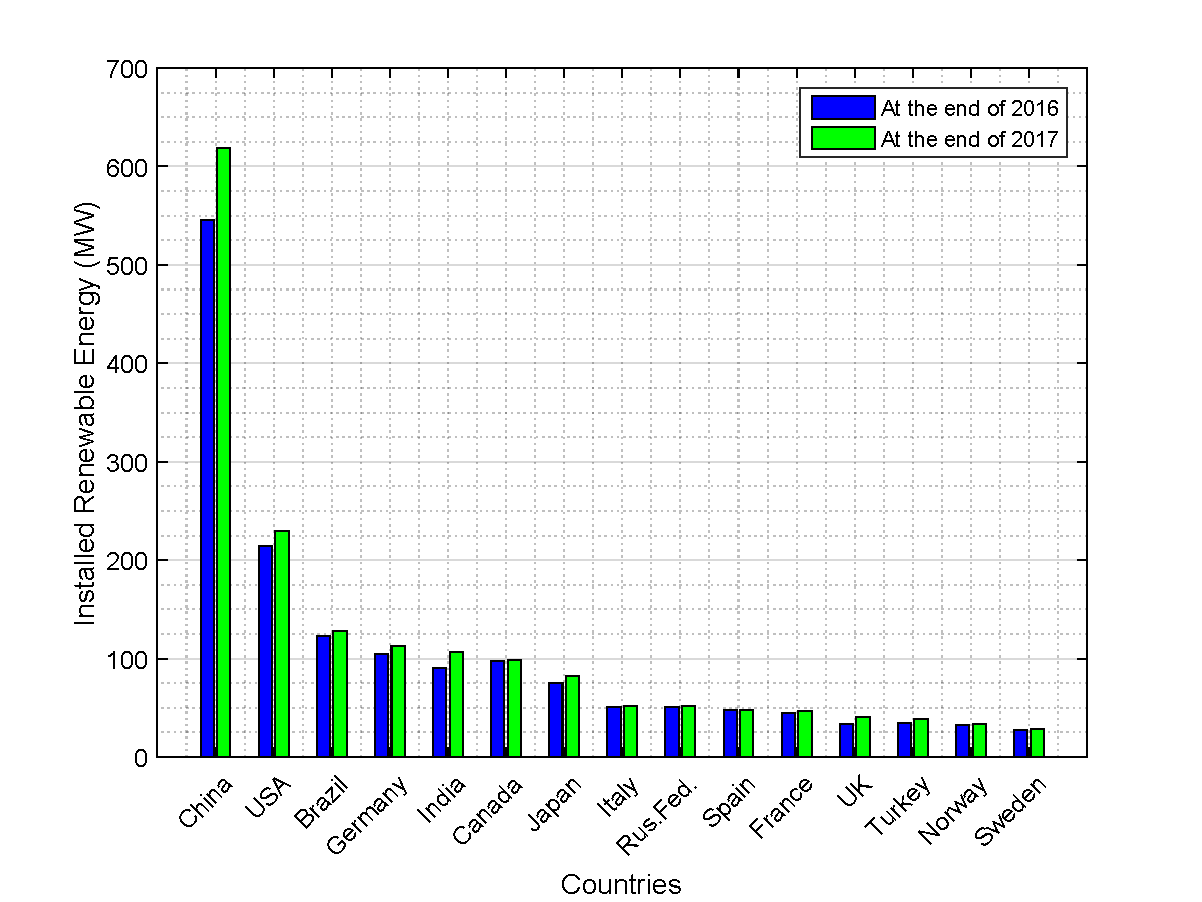
\includegraphics[scale=0.6]{renewablecapacities.pdf}
	\caption{Installed Renewable Energy Capacity of Leading Countries \cite{InternationalRenewableEnergyAgencyIRENA2018},\cite{InternationalRenewableEnergyAgency2017}}
	\label{renewablecap}
\end{figure}
EU countries promote the renewable energy systems from the very beginning. In 2008, two key main targets are set for 2020 by the European Council\cite{EuropeanCommission2008}: 
\begin{itemize}  
	\item At least 20 \% reduction in greenhouse gases (GHG) by 2020
	\item Achieving 20\% renewable energy share in energy consumption of EU by 2020
\end{itemize}
In order to accomplish these targets, the Renewable Energy Directive was published in 23 April 2009. This directive has set national binding targets for EU countries in order to accomplish the 20\% renewable energy target for EU and 10 \% target for the renewable energy usage in the transport \cite{EuropeanParliament2009}. In order to achieve the 20 \% target, each member state determined their own targets ranging from 10\% in Malta to 49\% in Sweden. According to the latest released report by Eurostat, renewable share of the EU in energy consumption has reached 17 \% in 2016 \cite{States2016}. Moreover, eleven of EU member states have already achieved their 2020 targets. Therefore, these ambitious targets imply that the increase in the renewable share will increase continuously.\par
Wind power has the highest share among the renewable energy sources in the installed renewable energy capacity except for hydro power. The wind power capacity at the end of 2017 has reached 514 GW worldwide\cite{InternationalRenewableEnergyAgencyIRENA2018}. The installed wind power capacity of the leading countries is shown in the Fig. \ref{windcap}. As in the case of total installed renewable energy capacity, China and USA have the highest installed capacities in the wind power capacity. \par
\begin{figure}[h!]
	\centering
	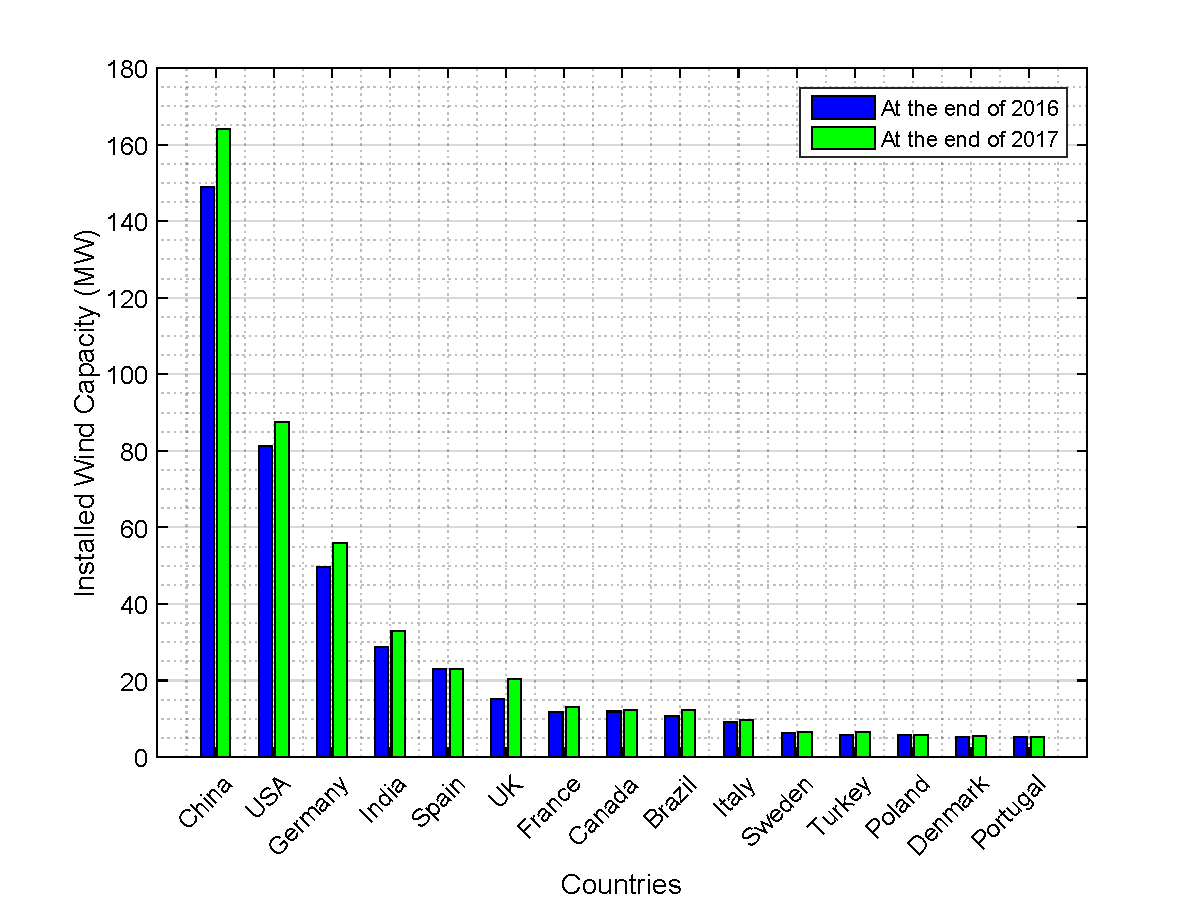
\includegraphics[scale=0.55]{windcapacity.pdf}
	\caption{Wind Power Capacity of Leading Countries in 2016 \cite{InternationalRenewableEnergyAgencyIRENA2018},\cite{InternationalRenewableEnergyAgency2017}}
	\label{windcap}
\end{figure}
The share of renewable energy is increasing continuously. Today, the discussion is about whether 100\% renewable energy is possible in the upcoming future. In \cite{REN212017d}, grid integration issues of wind and solar systems and the lack of sufficient storage technologies are considered as the main barrier for this target meanwhile the major problem seems as the existing energy industry. Nonetheless, a significant renewable share is expected even though the 100\% is realistic or not. The report published by IRENA (International Renewable Energy Agency) estimates the share of renewable energy in EU as 24\% by 2030 which is below proposed target of 27\%\cite{IRENA2014}. Nonetheless, the increase in the renewable energy share will continue in the upcoming future. \par
 
\section{Renewable Energy Problems}
It is an undeniable fact that renewable energy systems are advantageous in terms of global warming and carbon dioxide emission. Nonetheless, they also have disadvantages to the system operators due to intermittent energy generation profile. First of all, the term intermittent in the literature is related to the variable and uncontrollable nature of the renewable sources \cite{KlingeJacobsen2010}. Since the source of the Renewable Energy Sources (RES) is variable, it is not possible to adjust its output according to the demand. Therefore, the thermal plants have to be in the operation when high wind speeds and solar radiation exist. Moreover, the system requires additional start-ups and active power rise from partly loaded plants in order to balance the energy in the system because of the uncertainty of RES. These all create additional costs caused by high share of RES in the system \cite{Zipf2013}. Besides, power grid will face with transmission system issues as overloaded transmission lines, changes on the protection and control in the distribution system, greater level of power-factor control and low voltage ride-through (LVRT) requirements when the RES share is increased in the grid \cite{Ipakchi2009}.\par
Another challenge of increasing RES is the problem of power system frequency stability. Since the frequency of the power system depends on the balance between generation and consumption, grid operators are responsible for adjusting the generation in order to maintain a constant frequency. However, the renewable energy generation is strictly dependent on the renewable source i.e. solar radiation or wind speed. Therefore, renewable systems make the system operation harder due to their intermittent and uncertain power generation profiles. \par 
Frequency of the grid depends on the balance between supply and demand. As the balance is established, frequency stays constant. However, that is the ideal case. In fact, the load always varies. 
It is the responsibility of the grid operator to provide continues balance. Consequently, the grid frequency varies around the nominal frequency with small deviations. However, unintentional generation unit outages or instant load connections cause high deviations in the grid. A generic frequency disturbance is depicted in the Fig. \ref{freq2}. In the beginning of the disturbance, frequency falls with a slope that is called Rate of Change of Frequency (RoCoF) until the minimum frequency what is called frequency nadir is reached. Grid RoCoF is limited with the inertia of the generators. The higher grid inertia decreases RoCoF and increases the frequency nadir. \par
\begin{figure}[h!]
	\centering
	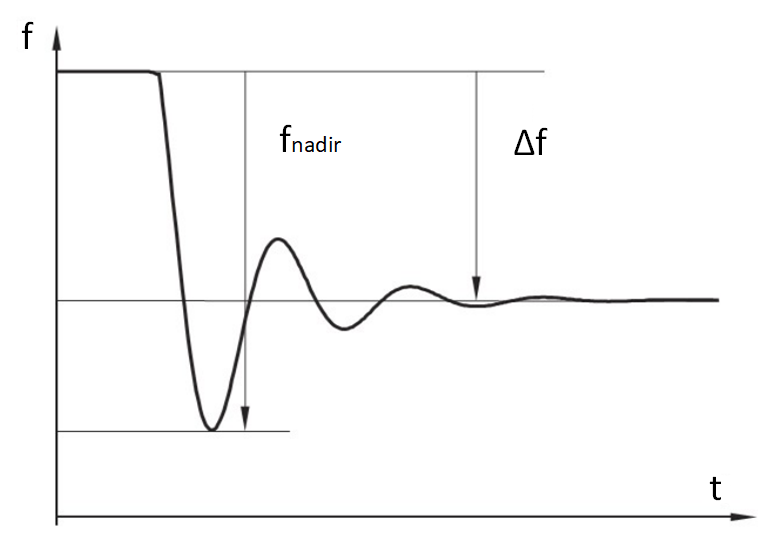
\includegraphics[scale=0.4]{freq2.png}
	\caption{A Generic Frequency Disturbance}
	\label{freq2}
\end{figure}
As the renewable systems with power electronics interface increase in the electricity grid, the grid equivalent inertia decreases. In \cite{Gautam2011}, the reduced grid inertia due to the high DFIG wind turbine penetration is emphasized. Moreover, the results of the reduced grid inertia following a disturbance are listed as: 
\begin{itemize}
	\item increased effective aggregated angular acceleration of synchronous machines which require high restoring forces
	\item high RoCoF and hence, decreased frequency nadir
\end{itemize}
It should be noted that this problem is not specific to DFIG wind turbines but renewable energy systems which are connected to the grid with power electronics. Conventional synchronous generators rotate at synchronous speed which is proportional to the grid frequency. If the grid frequency decreases, then the synchronous speed also decreases. In this case, the generator active power is increased inherently due to kinetic energy extraction from the generator inertia. The increase in active power provides action time for primary controllers and is crucial for frequency stability. \par
Different turbine topologies give different reactions to the frequency disturbances. Wind turbine generator topologies are shown in Fig. \ref{windtop}. Type-1 turbines are connected to grid with a asynchronous generator. The wind turbine generates active power as turbine rotates faster than synchronous speed. Therefore, the generator operates at the linear part of the torque-slip curve. Hence, the change in the grid frequency causes smaller decrease in the turbine speed. Type-2 is very similar to Type-1 except for the variable resistor which can shift the torque speed curve slightly. Hence, the frequency deviations affect the active power output of Type-1 and Type-2 \cite{Muljadi2012}. Type-3 wind turbines include Doubly-Fed Induction Generator (DFIG). DFIG stator is directly connected to grid meanwhile its rotor is connected to grid with a Partial Scale Power Converter (PSPC). Even though the stator is directly coupled to grid, the power electronics enable wind turbine to operate in a range of speeds. Therefore, the rotor frequency is also decoupled from grid.\par
\begin{figure}[h!]
	\centering
	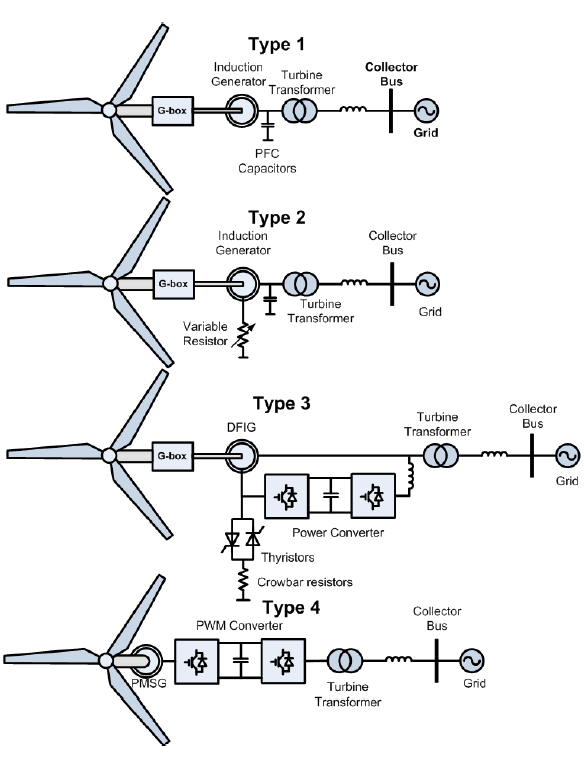
\includegraphics[scale=0.67]{windgentop.png}
	\caption{Wind Turbine Generator Configurations \cite{Muljadi2012}}
	\label{windtop}
\end{figure}
Type-4 wind turbines are connected to grid with back-to-back converters i.e. FSPC. AC/DC and DC/AC conversion decouples the grid frequency and the turbine speed. Due to the decoupling, Type-3 and Type-4 turbines can operate at the MPPT speed that capture the maximum power from air. Nonetheless, this results that Type-3 and 4 wind turbines are not affected from the grid frequency deviations. Therefore, these systems have no contribution to the grid inertia despite the fact that these systems include significant inertia. Hence, the aggregated grid inertia is reduced with the penetration of wind turbines with power electronics. \par
The comparison for different types of generators is made in \cite{VanDeVyver2016} and listed in Table \ref{generatorcomparison}. When the conventional synchronous generator is selected as reference, the fixed induction generator is marked as '+' meaning that it is affected by the grid frequency deviations. However, the grid frequency deviations have small impact on the rotational speed of the generator that decreases the inertial support behaviour. Moreover, DFIG wind generator is marked as '-' meaning that the speed of the generator is disturbed but no inertial support is provided. In this case, PSPC regulates the generator speed. Finally, the wind turbines with FSPC have no inertial response since the generator frequency is fully decoupled from grid frequency.
\begin{table}[h!]
	\centering
	\begin{tabular}{lc}
				\hline
		\multicolumn{1}{c}{\textbf{Type of the generator}}                                                                            & \textbf{Inertial Response Behavior} \\ \hline
		Conventional Synchronous Generator                                                                                            & ++                                   \\
		Fixed Speed Induction Generator (FSIG)                                                                                        & +                                    \\
		Doubly Fed Induction Generator (DFIG)                                                                                         & -                                    \\
		\begin{tabular}[c]{@{}l@{}}Variable Speed Wind Turbine Generator\\ (with Full Scale Power Electronics)\end{tabular} & None                                 \\ \hline
	\end{tabular}
	\caption{Comparison of Different Types of Generators for Inertial Response Behaviour}
	\label{generatorcomparison}
\end{table}
Another reason for the decrease in the grid inertia is the de-commitment or dispatch of the conventional sources due to economic concerns. Since the renewable energy systems have the lowest cost for energy production, they are preferred instead of conventional generators in the economical dispatch. As a result, conventional generators are dispatched to a lower generation profile or taken-off from operation.\par
It should be noted that grid inertia is directly related to the amount of load in the system in addition to the share of RES. Since the amount of online generators fluctuate within time, the grid aggregated inertia also changes. Hence, the scenario in which the system has low demand and also high renewable generation is the most critical one since the lowest grid inertia exists in the network.\par
In brief, the main problem that comes with increasing RES penetration is the reduction in the grid effective inertia. If the share of the RES increases continuously, the existing grid will be exposed the higher RoCoF and lower frequency nadir in the future. The solution of this problem is the emulation of the synchronous generator inertial support behavior on the RES. However, the capability of the wind turbine for inertial support behavior is not revealed for varying wind speeds. This thesis study focuses on the investigation of the inertial support limits on the wind turbines with FSPC in order to maximize the support power. Besides, the economical perspective of the inertial support is also examined from the energy provider perspective. In this way, the feasibility of the inertial support is also studied by focusing on the payment methods of the grid supporting applications. Consequently, maximum performance can be obtained from wind turbines that enables the power grid increasing the share of RES without causing frequency stability problems to grid operators.
\section{Literature Review}
Studies regarding inertial support date back to early 2000s. In the study \cite{Lalor2004}, the effect of the increasing wind energy penetration is investigated. The study concludes that increasing share of wind energy increases the primary reserve requirement for the successful grid operation. The increased frequency deviations, especially in light load conditions (high wind generation with low consumption scenario) can be mitigated in the system as long as the wind generation provides inertia support. Study in \cite{Ekanayake2003} states that DFIG wind turbines are decoupled from power system resulting in no contribution to system inertia. A supplementary loop is proposed for reinstating the machine inertia. Moreover, in \cite{Ekanayake2004}, performance of the  supplementary control loop is evaluated with the comparison of the inertial support of a fixed-speed wind turbine. The proposed control loop which is shown in Fig. \ref{inertiacontrol} is validated in \cite{Morren2006} and compared with the droop control in \cite{Morren2006a}.\par
\begin{figure}[h!]
	\centering
	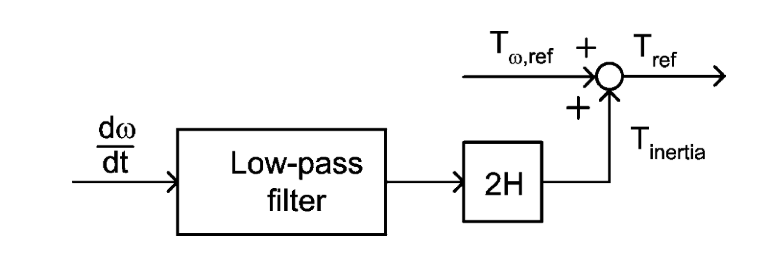
\includegraphics[width=.65\linewidth]{inertiacontrol.png}
	\caption[Inertia Controller]{Inertia Controller in \cite{Morren2006a}}
	\label{inertiacontrol}
\end{figure}
It is an undeniable fact that renewable energy systems are the most economical way of producing electrical energy due to absence of any fuel cost. Therefore, they are to be operated in their rated power. If they are required for the primary frequency control, the wind turbine active power should be curtailed. In this way they can leave a margin for droop control. Droop control by wind energy systems is also studied in the literature. In \cite{Muljadi2012}, the inertial support of different types of wind turbines is compared. It is concluded that the Type-4 wind turbines are able to perform better performance for inertial support due to the power electronics interface. Moreover, combination of inertial support and droop control produces better results in these wind turbines.\par
Inertial support by utilizing the kinetic energy in the turbine is proposed in literature with two main methods. One of the methods is increasing the active power by a defined percentage and it is presented in literature with different names such as Fast
Inertial Support, Fast Power Reserve or Stepwise Inertial Control. In this type of support, the support power is released with a step increase in the active power. In \cite{Hansen2014}, the fast inertial support is proposed with predefined increases in the active power. Nevertheless, the converter ratings and the effect of the wind speed in the fast inertial support capability are not emphasized. \par
The second proposed method is the active power increase proportional to grid RoCoF. The method is called in literature as synthetic inertia control, hidden inertia control or
virtual inertia. Actually, synthetic inertia is a method not only for wind turbines but converter interfaced systems to emulate synchronous generators. In \cite{Zhu2013a}, the method is implemented a VSC-HVDC system in order to improve frequency stability of a weak grid. Study \cite{Hernandez2017} focuses on the implementation in the PV systems in coordination with energy storage systems. In \cite{Zhu2018a}, the synthetic inertia implementation is studied with cooperation with Lithium-Ion supercapacitors. \par
In the studies \cite{VanDeVyver2016},\cite{Conroy2008},\cite{Gonzalez-Longatt2013}, the synthetic inertia controller is implemented on a variable speed wind turbines. The active power output of the wind turbine is changed according to the grid RoCoF as shown in the Fig. \ref{inertiacontrol2}. The effects of the synthetic inertia implementation in a full-scale wind turbine are studied in \cite{Gonzalez-Longatt2013}. A variable synthetic inertia controller is proposed in \cite{Bonfiglio2019} that improves the speed recovery of the wind turbine. Nonetheless, the better speed recovery is achieved at the expense of the longer speed recovery time. \par
\begin{figure}[h!]
	\centering
	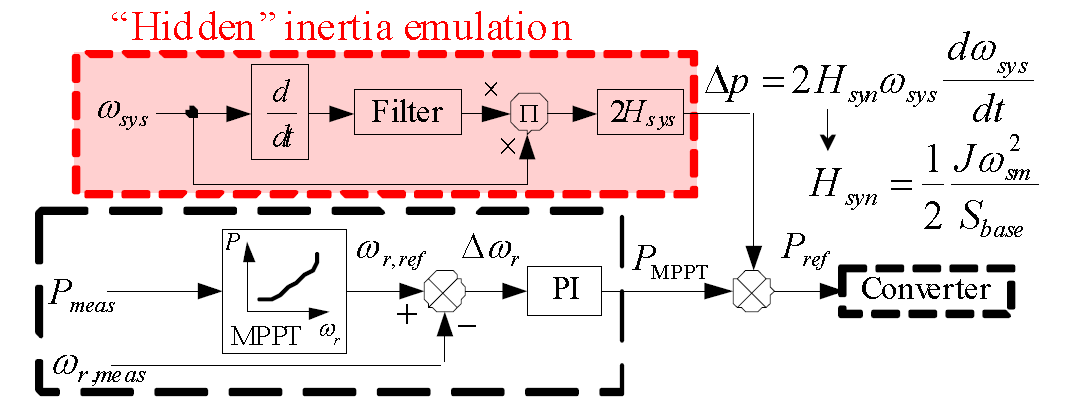
\includegraphics[width=.8\linewidth]{inertiacontrol2.png}
	\caption{Hidden Inertia Controller in\cite{Gonzalez-Longatt2013}}
	\label{inertiacontrol2}
\end{figure}
The modern wind turbine manufacturers also study the inertial support capability for their wind turbines. General Electrics has active power control module called as WindINERTIA for their wind turbines in order to react the large frequency disturbances. The control module can increase the power output of the wind turbine by 5-10\% for a few seconds (10\% for 15 seconds) \cite{Clark2009}. The control diagram of the module is shown in Fig. \ref{inertiacontrolge}. Moreover, Enercon provides inertial response capability to the turbines by allowing 10\% increase in the active power\cite{Enercon2018}. Nonetheless, solutions of GE and Enercon are independent of the grid RoCoF.\par
\begin{figure}[h!]
	\centering
	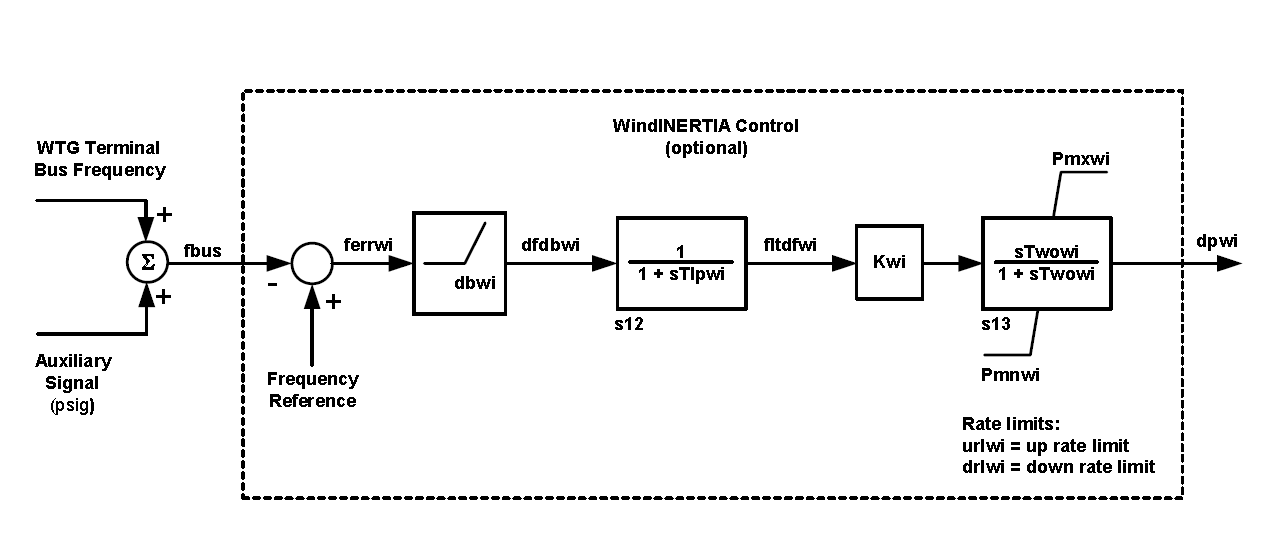
\includegraphics[width=.95\linewidth]{inertiacontrolge.png}
	\caption{GE WindINERTIA Control Diagram in \cite{Clark2009}}
	\label{inertiacontrolge}
\end{figure}
However, the full capacity of the wind turbines for inertial support is not studied in literature. Practical limits of the inertial support are studied in \cite{Gonzalez-Longatt2016} by varying the inertia constant to be emulated. The study focuses the emulation of higher inertia constants without consideration of the wind speed in the support time. The practical limits in terms of maximum achievable power and turbine internal parameters are not focused in the study. Finally, the studies in literature do not investigate the practical limits of the wind turbine. By investigating full capacity of the wind turbine, the importance of the wind turbines for frequency stability studies can be emphasized. 
\section{Thesis Motivation}
Although renewable energy systems are beneficial for environmental concerns and the absence of fuel cost, higher renewable penetration also brings operational challenges for system operators. One of the most important problems that comes with renewable energy is the deterioration on the power system frequency stability. With the high renewable penetration, grid aggregated inertia decreases. As a result, grid is exposed to high rate of change of frequency (RoCoF) for the disturbances in heavily renewable penetrated systems. This implies that the successful operation of power systems with increasing renewable energy penetration is not achievable unless the decrease in the grid inertia is prevented. Therefore, the main objective of this study is to avoid the decrease in the grid inertia arising with the renewable energy penetration. In this way, the share of renewable energy systems can be increased without the negative effects on the power system operation.

%To avoid steeper frequency declines in the grid, all generation technologies should provide inertial support for the frequency disturbances.\par
Wind energy systems, especially variable speed wind turbines with full scale power electronics are the most promising renewable energy systems that can contribute to grid frequency stability due to the high inertia in their blades and generator and also their back-to-back converters that give ability to control its active power. Wind turbine with full-scale power electronics is the key solution to be used against the decrease in the grid inertia. However, the full capability of a wind turbine with full-scale power electronics has not been discovered yet. This study will explore the full capacity of the wind turbines for the inertial support. The practical limits of the wind turbines are explored under different wind speed scenarios. Another objective of this study is revealing the effects of grid supporting functions in the wind turbines. Besides, the differences between the frequency dependent and independent inertial support mechanisms are investigated especially for weak power systems.
%The knowledge of the wind turbine inertial support capability enables the grid operator to build new frequency regulating mechanisms. In this way, the participation of turbines for these mechanisms can be encouraged. \par
%Inertial support methods (either dependent on frequency or not) are presented in the literature. However, comparison of their performances under a weak power grid has not studied. This study aims to find out which type of inertial support is efficient for weak power grids. \par
%In Turkey, renewable energy systems produce electricity through the feed-in tariff that is the guaranteed price to these systems. Hence, the energy providers would not be volunteer for inertial support implementation unless system operators make this service mandatory or the implementation has economical benefits. The results of this thesis will present a basis for economical analysis by the energy provider perspective.
\section{Thesis Outline}
This thesis study focuses on the wind turbine inertial support limits and its effects on power system stability. The thesis starts with a brief summary of the renewable energy status in Chapter \ref{chp:1}. By reviewing the share of the renewable energy systems and the targets for upcoming future, the importance of the frequency stability studies is highlighted. Moreover, renewable energy problems and the proposed solutions in literature are presented. \par
In Chapter \ref{chp:2}, the frequency concept in power systems is extensively described. Since renewable energy systems are replaced or preferred over the conventional power generation units, the electricity grid is facing with frequency stability issues due to the absence of inertia-less units. Therefore, the behaviur of old-fashion power plants are described under frequency disturbances. Moreover, the frequency regulating mechanisms are presented. Finally, the energy markets are also explained in order to emphasize the position of renewable energy systems.\par
Chapter \ref{chp:3} presents the modelling of wind turbine used in this study. Since the existing variable speed wind turbines require modification in order to integrate to electricity grid, detailed modelling of these wind turbines is presented. By utilizing synthetic inertia method, a relation between grid frequency and the active power output is constructed.\par
The limits of the active power increase are investigated in Chapter \ref{chp:4}. The ability of increasing its active power output is already presented in literature. However, the limits of support power are studied for different wind speed scenarios. The real wind speed measurements from site are utilized to find the probability of support power for different wind speeds. Wind turbine inertial support limits and turbine internal parameters are observed for the non-dynamic frequency response.\par
Synthetic inertia implementation is the implementation of inertial support behavior on RES by establishing a relation between grid RoCoF and turbine active power output. The implementation on a wind farm is studied in Chapter \ref{chp:5}. The effect of synthetic inertia is observed in a dynamic test case with renewable penetration. Test case is modified with different combinations in which the system is penetrated with wind farm with/without generator decommission are studied in this chapter. Frequency response of the test system is tested for different grid configurations as well as different emulated inertia constants. Furthermore, the synthetic inertia implementation is evaluated for the Turkish electricity system. \par
Chapter \ref{chp:6} evaluates the effects of the fast inertial support and synthetic inertia implementation. Moreover, an economical analysis from an energy provider perspective is given. Two hypothetical payment methods are constructed and compared to estimate which economical motive can convince the energy provider for participating grid supporting methods with renewable energy systems. \par
Chapter \ref{chp:7} presents a basic conclusion for the inertial support implementation which is either frequency dependent or not. The contribution of the thesis study on the grid inertia reduction is emphasized by reviewing the inertial support capability of the wind turbine especially for low and medium wind speeds. Moreover, the feasibility of the inertial support implementation is investigated in terms of the payment methods.


















% CHAPTER 1
\chapter{POWER SYSTEM FREQUENCY STABILITY}
\label{chp:2}
The increasing renewable energy penetration deteriorates the power system frequency stability. One of the most severe effect of renewable energy penetration is the reduction in grid inertia. Grid aggregated inertia is important for the frequency stability. As the frequency falls, a part of the kinetic energy is extracted from the grid inertia and released inherently from synchronous generators to grid. Therefore, as the grid aggregated inertia decreases, the control of the frequency becomes difficult resulting in quick changes in the grid frequency.\par
In this chapter, the internal dynamics of the power system will be presented in terms of frequency stability. The frequency regulation mechanisms in the grid is presented. Furthermore, the energy market is briefly explained in order to understand the role of renewable energy providers inside the market.
\section{Synchronous Generator and Synchronous Speed}
Synchronous machines produce torque only in synchronous speed. If a transient over-speeding occurs in the rotor, the torque cannot be produced that results in a deceleration. This makes the rotor angular velocity to strictly coupled to the electrical frequency  of the stator rotating MMF. This is why these machines are equipped with damper windings which are basically induction machine windings. If the frequency of  grid changes, damper windings create a torque which creates a force to synchronize the speed to the grid frequency. \par
\begin{equation}
n_{s}=\frac{120f}{p}
\label{syncspeed}
\end{equation}
Relation between grid frequency and the synchronous speed is given in Eq. (\ref{syncspeed}) in terms of rpm where $n_{s}$ is the synchronous speed in rpm, $f$ is the grid frequency in Hz, $p$ is the number of poles of the generator \cite{Kundur}.

\section{Swing Equation}
\label{swing}
Rotational speed of synchronous machines changes according to the net torque acting on the rotor. Therefore, the speed is maintained constant unless there is a difference between mechanical and electromechanical torque. The equation of motion is given in Eq. (\ref{eqmotion}) where $J$ is aggravated moment of inertia of the generator and the turbine in $kgm^{2}$, $\omega_{m}$ is the rotor angular velocity in $rad/s$, $T_{m}$ and $T_{e}$ are mechanical and electromechanical torques in $Nm$. $T_{a}$ is the accelerating torque in $Nm$ which determines the acceleration or deceleration in the rotor according to its sign.
\begin{equation}
J\frac{d\omega_{m}}{dt}=T_{m}-T_{e}=T_{a}
\label{eqmotion}
\end{equation}
In power system network, the power ratings of the generators in operation and corresponding moment of inertia values varies. Inertia constant is defined as the ratio of kinetic energy stored in the inertia to the power rating of the generator as in Eq. (\ref{inertiaconstant}) where $\omega_{0m}$ denotes the rated angular velocity of generator in $rad/s$ and $S_{base}$ is the rated apparent power in $VA$. $H$ is indicates the time duration in which generator produces its rated apparent power by only using its kinetic energy in the inertia. Thus, $H$ is a better indication of factor for power system frequency stability analysis compared to $J$. Hence, it is more convenient to use inertia constant, $H$ which varies between 2 and 9 seconds \cite{Kundur}.
\begin{equation}
H=\frac{{\frac{1}{2}}J\omega_{0m}^{2}}{S_{base}}
\label{inertiaconstant}
\end{equation}
Substituting Eq. (\ref{inertiaconstant}) into Eq. (\ref{eqmotion}) and replacing units to per-unit quantities yield the swing equation given in Eq. (\ref{eqmotion5}) where $\overline{P_{m}}$ is the input mechanical power in pu and $\overline{P_{e}}$ is the electromechanical output power in pu. It defines the inherent behaviour of a synchronous generator against the frequency deviations in the grid. When the grid frequency falls, a subsequent decrease in the rotor is observed. According to the Eq. (\ref{eqmotion5}), a negative term is found in the left-hand side. This means that rotor electromechanical output power, $\overline{P_{e}}$ will be increased inherently. It should be noted that the additional energy is not taken from the input mechanical power but it is extracted from the kinetic energy. Moreover, the decreased energy is injected to grid whenever the frequency increases due to the acceleration in the rotor.
%\begin{equation}
%J=\frac{2H}{\omega_{0m}^{2}}{S_{base}}
%\label{inertiaconstant2}
%\end{equation}
%\begin{equation}
%\frac{2H}{\omega_{0m}^{2}}{S_{base}}\frac{d\omega_{m}}{dt}=T_{m}-T_{e}
%\label{eqmotion2}
%\end{equation}
%\begin{equation}
%\frac{2H}{\omega_{0m}^{2}}{S_{base}\omega_{m}}\frac{d\omega_{m}}{dt}=P_{m}-P_{e}
%\label{eqmotion3}
%\end{equation}
%\begin{equation}
%2H\frac{\omega_{m}}{\omega_{0m}}\frac{d(\omega_{m}/\omega_{0m})}{dt}=\frac{P_{m}-P_{e}}{S_{base}}
%\label{eqmotion4}
%\end{equation}
\begin{equation}
2H\overline{\omega_{m}}\frac{d\overline{\omega_{m}}}{dt}=\overline{P_{m}}-\overline{P_{e}}
\label{eqmotion5}
\end{equation}
\section{Frequency in Power Systems}
The frequency in a power system is related to the speed of the synchronous generators and changes according to the swing equation. The frequency of the each generator is not the same in the network since each generator does not have the same speed. Nonetheless, the fluctuations in the generator speeds are called rotor swings and can be negligible in the steady state. Hence, the network can be assumed as a single generating unit by neglecting small differences between the generator speeds. The swing equation basically investigates the relation between mechanical and electromechanical powers and the rate of change of angular speed of a generator. However, it is also applicable to grid in order to estimate the grid frequency.\par
\begin{equation}
\label{systemswing}
2H_{sys}\overline{f}_{sys}\frac{d\overline{f}_{sys}}{dt}=\overline{P}_{tm}-\overline{P}_{te}
\end{equation}
If the generators of the grid is considered as a single generator, the inertia of the equivalent generator is aggravated from each generator in the network. In this case, average frequency in the network can be found as in Eq. (\ref{systemswing}) where $P_{tm}$ is the aggravated mechanical input power of the generators meanwhile $P_{te}$ is the aggravated electromechanical output power. In other words, the system frequency depends on the balance between generation and consumption. It should be noted that generation means the input mechanical power of the generators meanwhile the demand is absorbed from the electromechanical output power of the generators. Hence, the difference between these causes either acceleration or deceleration. \par
\begin{figure}[h!]
	\centering
	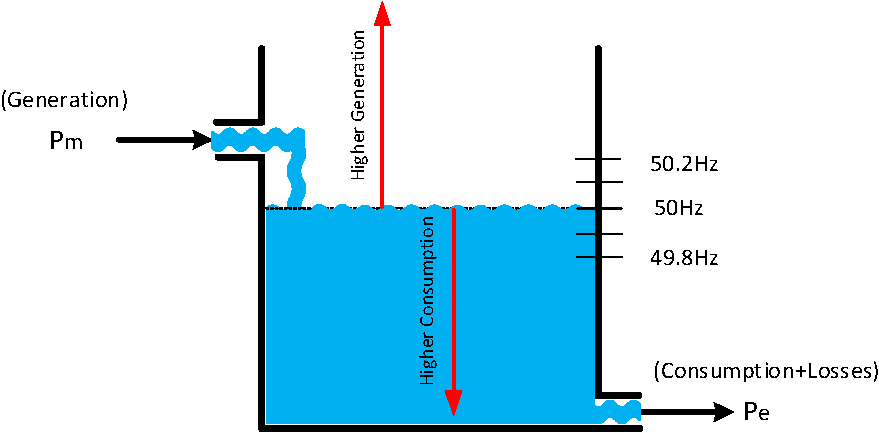
\includegraphics[width=.9\linewidth]{frequencypool.pdf}
	\caption{Frequency behaviour in electric grid with the water level in a container analogy \cite{Eto2010}}
	\label{frequencyingrid}
\end{figure}
The behaviour of the frequency in electric grid is depicted in Fig. \ref{frequencyingrid}. As it can be seen from the water level in a container analogy, the frequency of the system is dependent on the in-flow and the out-flow. Therefore, in the electricity grid, frequency increases as the aggravated input power is higher than the aggregated output power. Note that, the direction of the frequency is dictated by this balance. Having a constant 49.8Hz frequency does not mean that consumption is higher than generation. If the frequency is constant, then the input mechanical power is equal to output power.\par
The variation of the grid frequency is depicted for a typical day in Fig \ref{06decfreq}. The frequency deviates continuously during the day. It should be noted that there exists hourly peaks in the frequency. The peaks occur due to the change in the hourly generation shift. Since the generation level is changed for the next hour, the frequency deviates hourly in the grid.
\begin{figure}[h!]
	\centering
	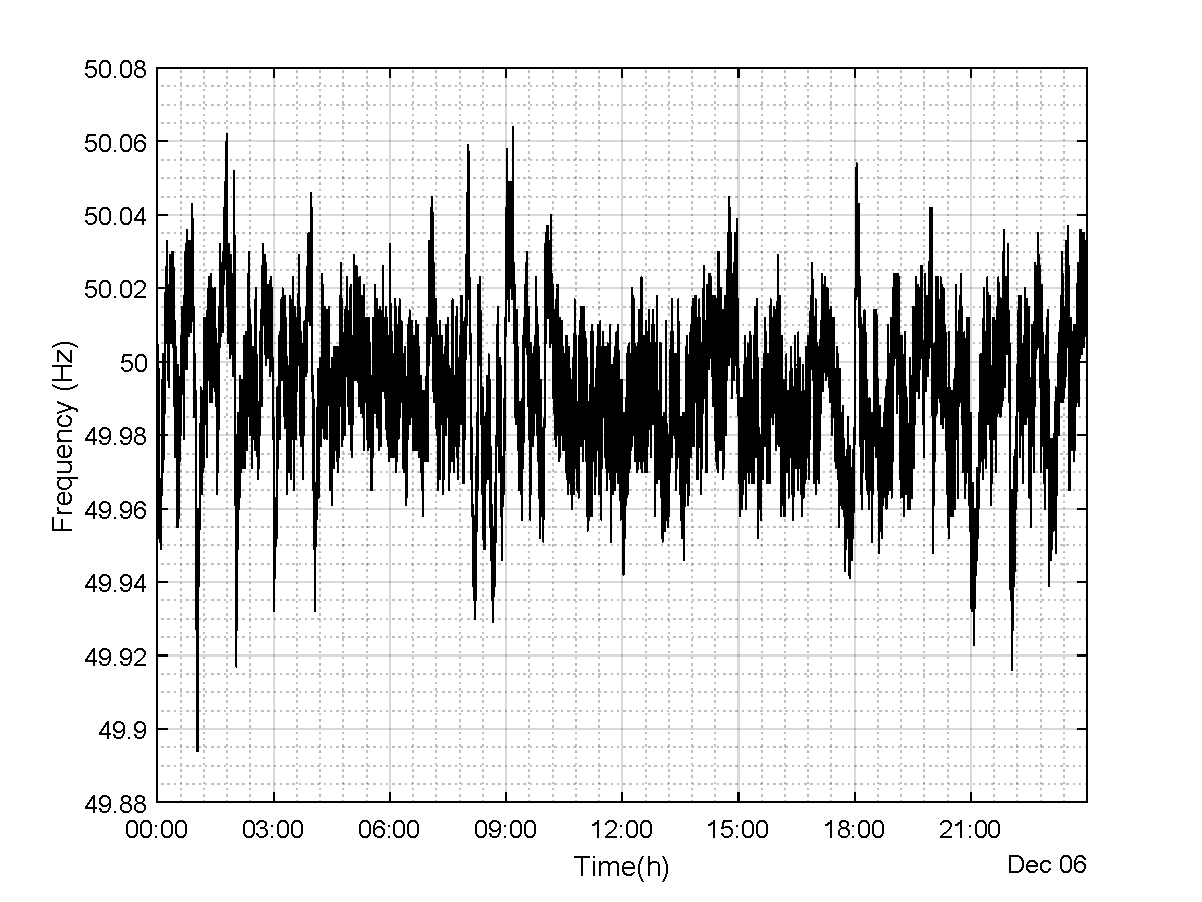
\includegraphics[width=.9\linewidth]{06decfreq.pdf}
	\caption{Variation of the Frequency in a Typical Day (06 Dec 2018) \cite{teiasfreq}}
	\label{06decfreq}
\end{figure}
\section{Frequency Regulating Mechanisms}
Having a constant frequency is one of the most important responsibilities of a system operator. In order to have a constant frequency, supply is being adjusted according to the demand continuously. By doing so, the system frequency varies between a band-gap. The variation depends on the disturbances which are generally a sudden generation outage or instant load connection. The size of the disturbance determines the severity of the frequency change and there are three main mechanisms to arrest the frequency changes in the system. \par
The frequency control services in England and Wales are depicted in Fig. \ref{freqcontrol} for a frequency disturbance. The frequency is maintained between 49.8Hz and 50.2Hz for continuous service. A frequency disturbance event causes frequency to decline. However, the decline in the frequency is arrested with the help of the inertial support of the conventional generators and the primary frequency controllers. The main responsibility of the primary frequency control is arresting the frequency decline. Restoration of grid frequency to nominal is the responsibility of the secondary and tertiary frequency controls.
\begin{figure}[h!]
	\centering
	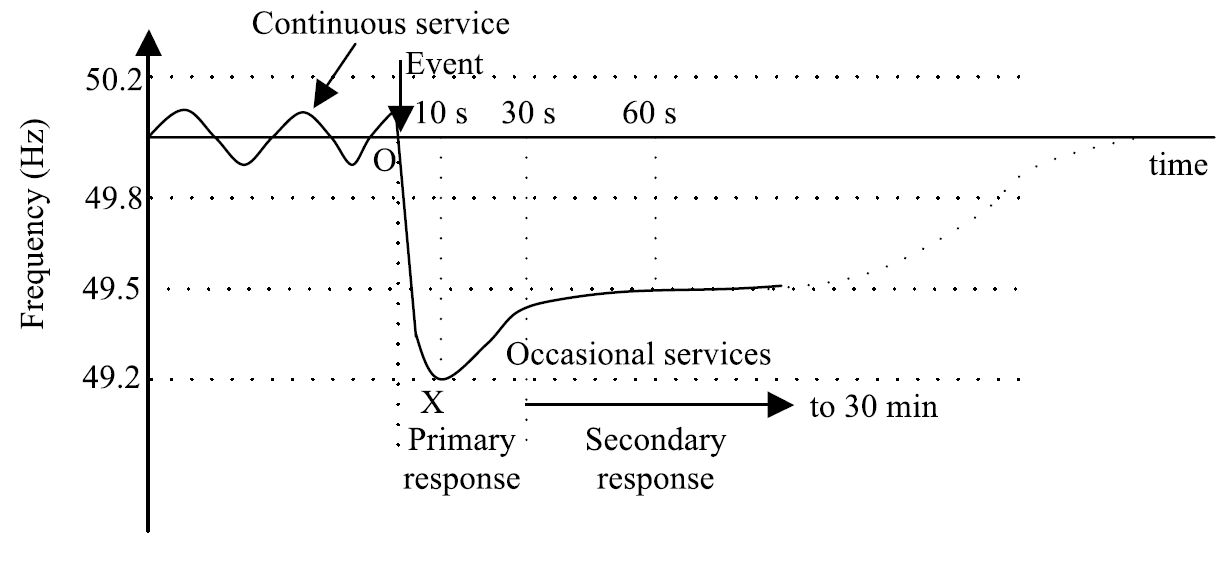
\includegraphics[scale=0.35]{freqq.png}
	\caption{Grid Frequency Control in England and Wales \cite{Ekanayake2008}, \cite{Erinmez1999}}
	\label{freqcontrol}
\end{figure}
\subsection{Primary Frequency Control}
Following generator outage or sudden load connection event, frequency starts decreasing. The rate of change of the frequency is dependent on the severity of the event by means of power and the available inertia of the power system. Such frequency disturbance requires increased input power. However, the increase in the input mechanical power should be activated very fast and should be automated. This responsibility is assigned to generating units with primary frequency control. The active power generation of these units is increased or decreased by the governor depending on the network frequency direction. Notice that each generator in the power system does not necessarily perform primary frequency control function. In this case, their active power generation is independent from the network frequency. The contribution to primary frequency control is an responsibility but also a way to sell higher energy to grid operator.
The primary frequency control is automated with droop control defined in the generator speed governors. According to droop control, the generator power should be increased according to the frequency deviation from nominal. Therefore, the generating unit does not utilize its whole capacity but rather keeps a capacity which is called as spinning reserve. According to the droop curve, the generation unit should increase its output power no longer than 15 seconds and keep their operation up to 30 minutes\cite{Machowski2011}.
\subsection{Secondary Frequency Control}
The frequency is recovered back to nominal value with the Secondary Frequency Control action. This controller might be a single or multiple centres that monitor the frequency and adjust the generation accordingly. They are also called as Automatic Generation Control (AGC) systems and their action takes a few minutes. The AGC monitors the frequency deviation from the nominal and takes action to recover frequency back to nominal. With the secondary frequency control action, primary controllers decreases their production back to their pre-disturbance value.
\subsection{Tertiary Frequency Control}
The final frequency control mechanism is the Tertiary Frequency Control. If the frequency is not recovered back to nominal value with the secondary controllers, tertiary frequency controllers manually activates the load shedding which is an undesired situation by the network operator. However, it is an emergency case which might result in black-out and requires immediate action.
\section{Energy Market}
Since the energy is generated and distributed by private energy companies, a system operator should be responsible for maintaining a balance in the power network. The frequency is kept inside the operational band in the electricity network by balancing the supply and the demand by intersecting the supply and demand curves inside the different time intervals. In this way, the balance is ensured in the market by day ahead, intra-day and balancing markets. 
\subsection{Day Ahead Market}
The load power in a network has a distinct characteristic depending on the day of the week or the hour of the day. By foreseeing the next day demand power variation, the electricity market collects the bids from the energy suppliers and consumers. According to submitted bids, the next day generation price is determined by intersecting the supply and demand price curves. The price of the energy is called Market Clearing Price (MCP). These bids are submitted for the next day and the prices are determined before the corresponding day.
\subsection{Intra-Day Market}
Even though the estimations for the upcoming day load power has superior accuracy with the advanced estimation methods, networks are subjected to unexpected problems such as generator trips, line outages. Therefore, intra-day market contributes the balance of the market between the day ahead market and balancing market. Moreover, it gives the participants almost real-time trading opportunity meanwhile it increases the sustainability of the market. After day ahead market has closed for the corresponding day, the bids are submitted to system. In other words, MCP is already determined for the corresponding day meanwhile the rest of the day prices are not set. 
\subsection{Balancing Market}
Primary and secondary control reserves are maintained in the system in order to improve the balance for the instant deviations in the frequency. The frequency is first arrested by the primary controllers and it is restored by the secondary controllers. The generation units that participate primary and secondary control promises a defined generation capacity to these actions. Balancing market is much more different than day ahead and intra-day market since its main goal is the network security rather than electricity trading. The price of the energy in this market called as System Marginal Price (SMP).\par
The price of the energy changes according to the market type. In the Fig. \ref{markets}, three market prices such as Market Clearing Price (MCP), Weighted Average Price (WAP) and System Marginal Price (SMP) are shown.
\begin{figure}[h!]
	\centering
	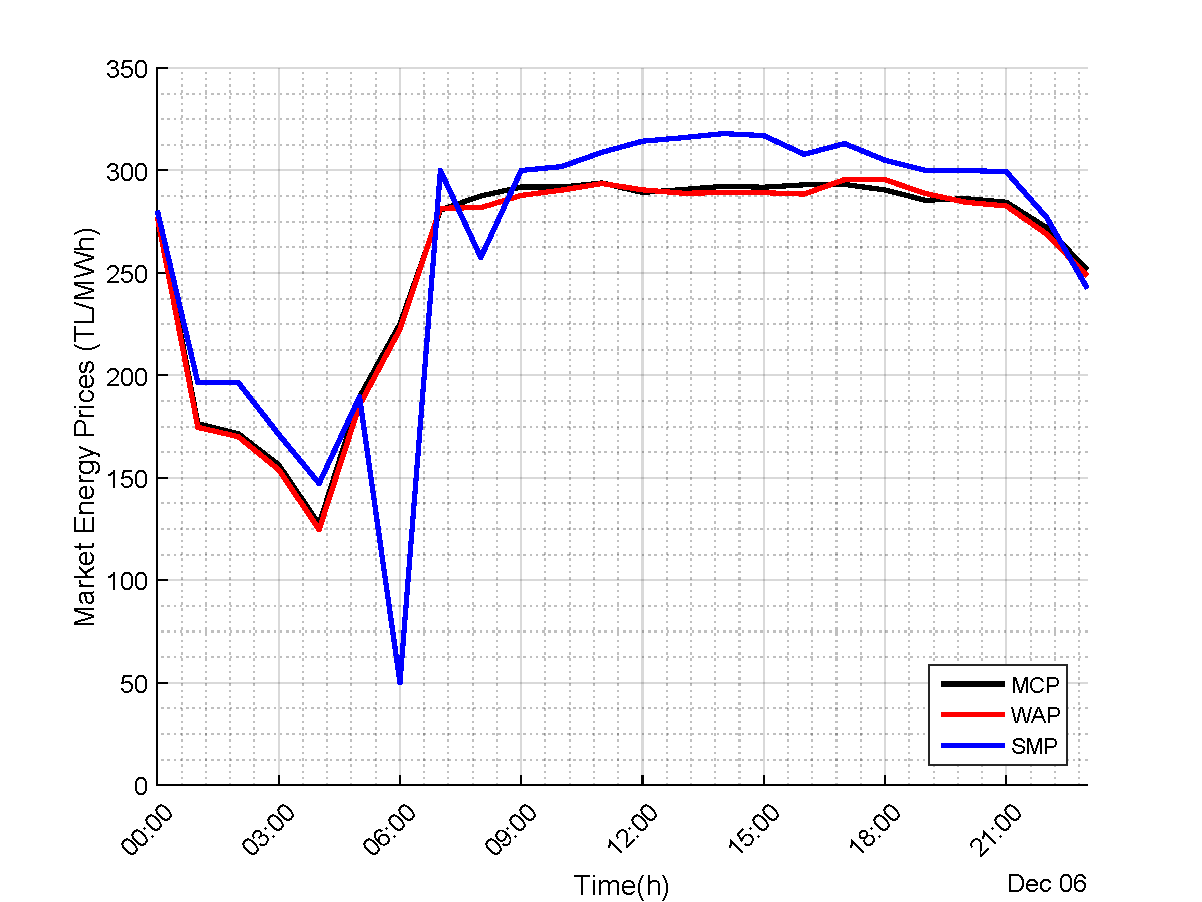
\includegraphics[scale=0.7]{marketprices.pdf}
	\caption{Energy Prices on 06 Dec. 2018 \cite{TEIAS2019}}
	\label{markets}
\end{figure}
\subsection{Feed-In Tariff}
\label{section-price}
Significant amount of energy produced inside the Turkish electricity network is based on exported sources such as coal and gas. As a result of this, the energy sector is highly dependent on the foreign countries. In order to decrease the dependency on the external sources, the renewable energy sources are supported by government in Turkey. The energy generated by renewable energy systems are bought with the feed-in tariff (FIT) within the pre-determined time interval according to the purchase agreement. This decreases the return of investment due to the fact that all produced energy will be bought during this period with a remarkable price. The feed-in tariff for different renewable energy systems is listed in Table \ref{price}.\par
\begin{table}[h]
	\centering
	\begin{tabular}{cc}
		\hline
		\textbf{Renewable Energy System} & \textbf{\begin{tabular}[c]{@{}c@{}}Feed-In Tariff\\ (cent/kWh)\end{tabular}} \\ \hline
		Hydro                            & 7.3                                                                          \\
		Wind                             & 7.3                                                                          \\
		Geothermal                       & 10.5                                                                         \\
		Biomass                          & 13.3                                                                         \\
		Solar                            & 13.3                                                                         \\ \hline
	\end{tabular}
\caption{Feed-In Tariff for Renewable Energy Systems in Turkey \cite{yasa}}
\label{price}
\end{table}
In addition to feed-in tariff, energy provider can benefit from additional incentives as long as some parts of the system is produced inside Turkey. For instance, by preferring the tower of a wind turbine which is a domestic production, an additional price is given to energy provider as local-bonus content. The local-bonus contents for wind turbines are listed in Table \ref{price2}.\par
\begin{table}[h!]
	\centering
	\begin{tabular}{cc}
		\hline
		\textbf{\begin{tabular}[c]{@{}c@{}}Local Content\\ for Wind Turbines\end{tabular}}   & \textbf{\begin{tabular}[c]{@{}c@{}}Local Content Incentive\\ (cent/kWh)\end{tabular}} \\ \hline
		Blade                                                                                & 0.8                                                                                   \\
		\begin{tabular}[c]{@{}c@{}}Generator and \\ Power Electronics\end{tabular}           & 1.0                                                                                   \\
		Turbine Tower                                                                        & 0.6                                                                                   \\
		\begin{tabular}[c]{@{}c@{}}All Mechanical Parts in \\ Rotor and Nacelle\end{tabular} & 1.3                                                                                   \\ \hline
	\end{tabular}
	\caption{Local Content Incentives for Wind Turbines\cite{yasa}}
	\label{price2}
\end{table}
With the increasing renewable energy penetration, the power system stability is getting more vulnerable to the disturbances. Since the grid operators are responsible for the successful operation of the grid, they work on grid stability improving. Nonetheless, power system stability is not the responsibility of the energy providers. However, participation of the renewable energy providers is also a necessity to improve frequency stability of the grid. Hence, the grid operators have to come up with a solution to be implemented by the energy providers. Nonetheless, the solution should also be beneficial for the energy providers who is already satisfied with the existing purchase agreement with additional incentives. As long as the renewable energy providers are convinced to implement the solutions, the grid stability can be maintained against the increasing renewable penetration.
\section{Conclusion}
This chapter focuses on the frequency dynamics inside the power grid. The importance of inherited inertial support of the synchronous generators are highlighted. The characteristics of this behaviour is defined with swing equation that can be adopted to renewable energy systems. The swing equation explains the change in the active powers of the synchronous generators upon a frequency disturbance on the output terminal. However, the internal dynamics of the frequency is also presented to understand the frequency stability. \par
Frequency regulating mechanisms such as primary, secondary and tertiary control are essential for power systems. Their action sequence are also explained in detail. In addition to technical details, the energy market is also summarized to present a economical perspective. 
% CHAPTER 1
\chapter{WIND TURBINE MODELLING}
\label{chp:3}
Ancillary services are getting attention especially for renewable energy systems. Participation of renewable energy systems to frequency regulating mechanisms will be a necessity for the successful operation of the power system. Hence, the detailed modelling of renewable energy systems are essential for grid supporting implementations. In this chapter, detailed modelling for wind turbines is investigated. The wind turbine modelling is presented for the wind turbines that are connected to grid with full-scale power electronics. 
\section{Wind Turbines with Full Scale Power Electronics}
The share of variable speed wind turbines with full scale power electronics is increasing worldwide due to the high efficiency. Full-scale power electronics enables the turbine to have wide speed range. The wind turbines in this type are able to adjust its speed according to the variation in the wind speed and torque \cite{Chen2009b}. PMSG wind turbines are one of the most common type of these turbines. Even though the price of the permanent magnet fluctuates with time, the reliability and high efficiency of this type of turbine increase its share in the market. The wind turbine modelling in this study is based on PMSG wind turbines. However, the ability to control the wind turbine output power is not just specific to PMSG wind turbines but the ones with full-scale power electronics. \par
Fig. \ref{varspeedpmsg_1}, \ref{varspeedpmsg_2} and \ref{varspeedpmsg_3} show the modelling of wind turbine topologies that are connected to grid full-scale back-to-back converter. In wind turbines with full-scale power electronics, stator of the wind turbine generator is not directly connected to grid. A back-to-back converter is used between generator and the electrical grid to ensure that the turbine speed is independent from the grid frequency. The back-to-back converter is composed of two converters to perform the AC/DC and DC/AC conversion. The converter which is connected to turbine generator is called Machine Side Converter (MSC) meanwhile the one connected to grid is called Grid Side Converter(GSC). Moreover, GSC is connected to grid with a filter in order to filter out high frequency currents due to switching action. Since GE2.75-103 model geared PMSG wind turbine model is used in this study, the turbine topology in Fig. \ref{varspeedpmsg_1} is emphasized. The turbine is composed of sub-models such as aerodynamic model, gearbox, PMSG, MSC and GSC. The details of the sub-models are given in the following sections.\par
\begin{figure}[h!]
	\centering
	\begin{subfigure}{0.9\textwidth} % width of right subfigure
		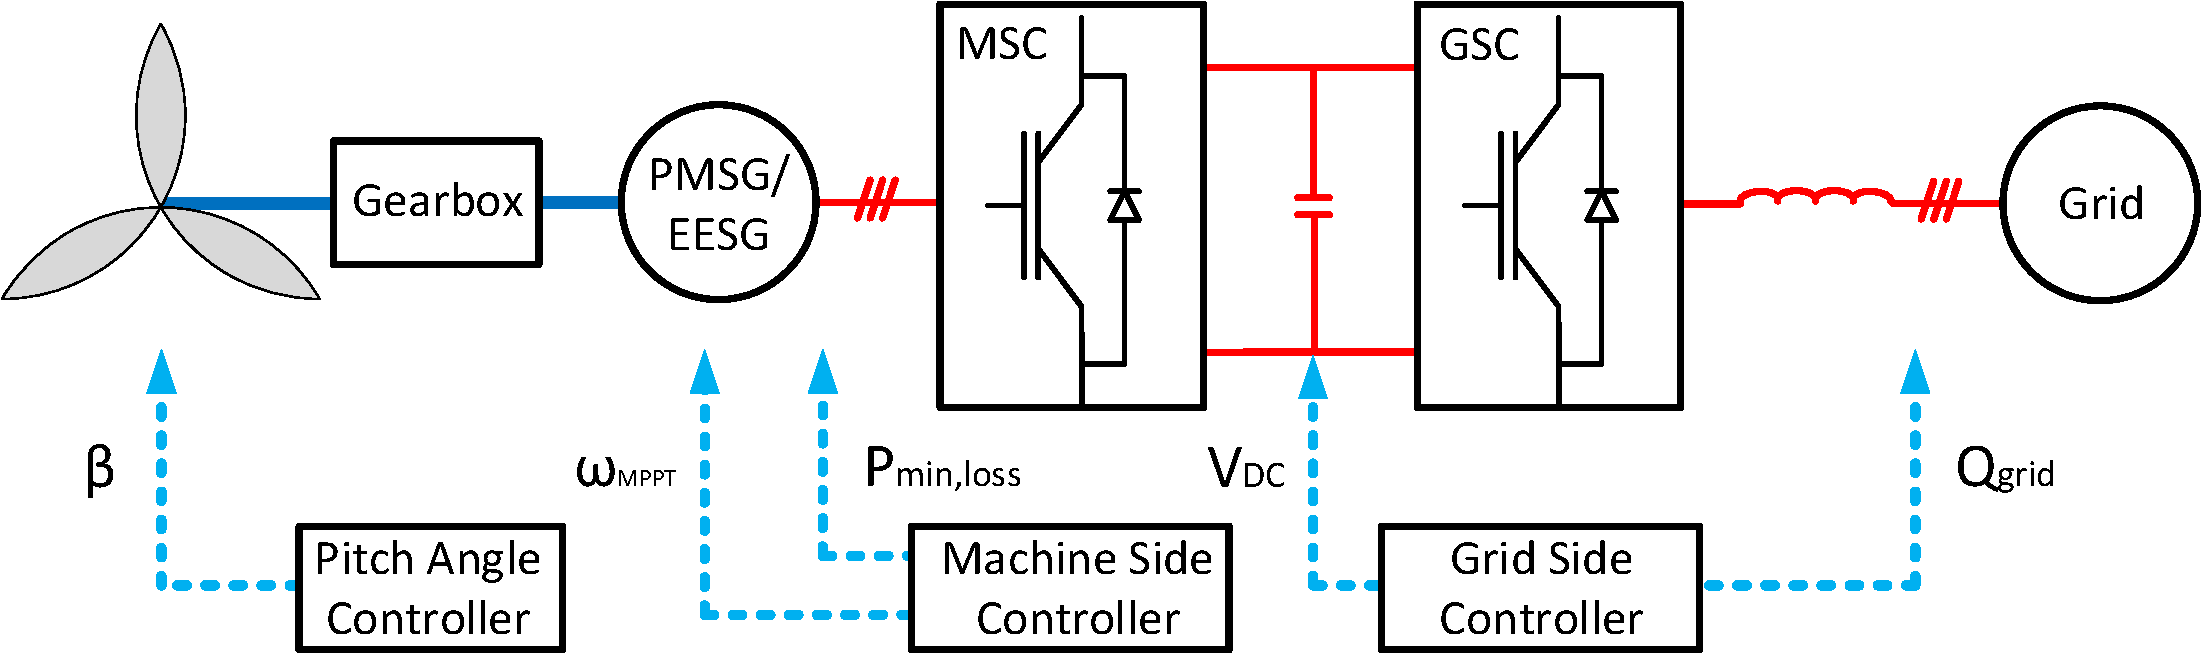
\includegraphics[width=0.9\linewidth]{windmodel2_1.pdf}
		\caption{Geared PMSG/EESG Wind Turbine}		
		\label{varspeedpmsg_1}
	\end{subfigure}
	\vspace{0.1em} % here you can insert horizontal or vertical space
	\begin{subfigure}{0.9\textwidth}
		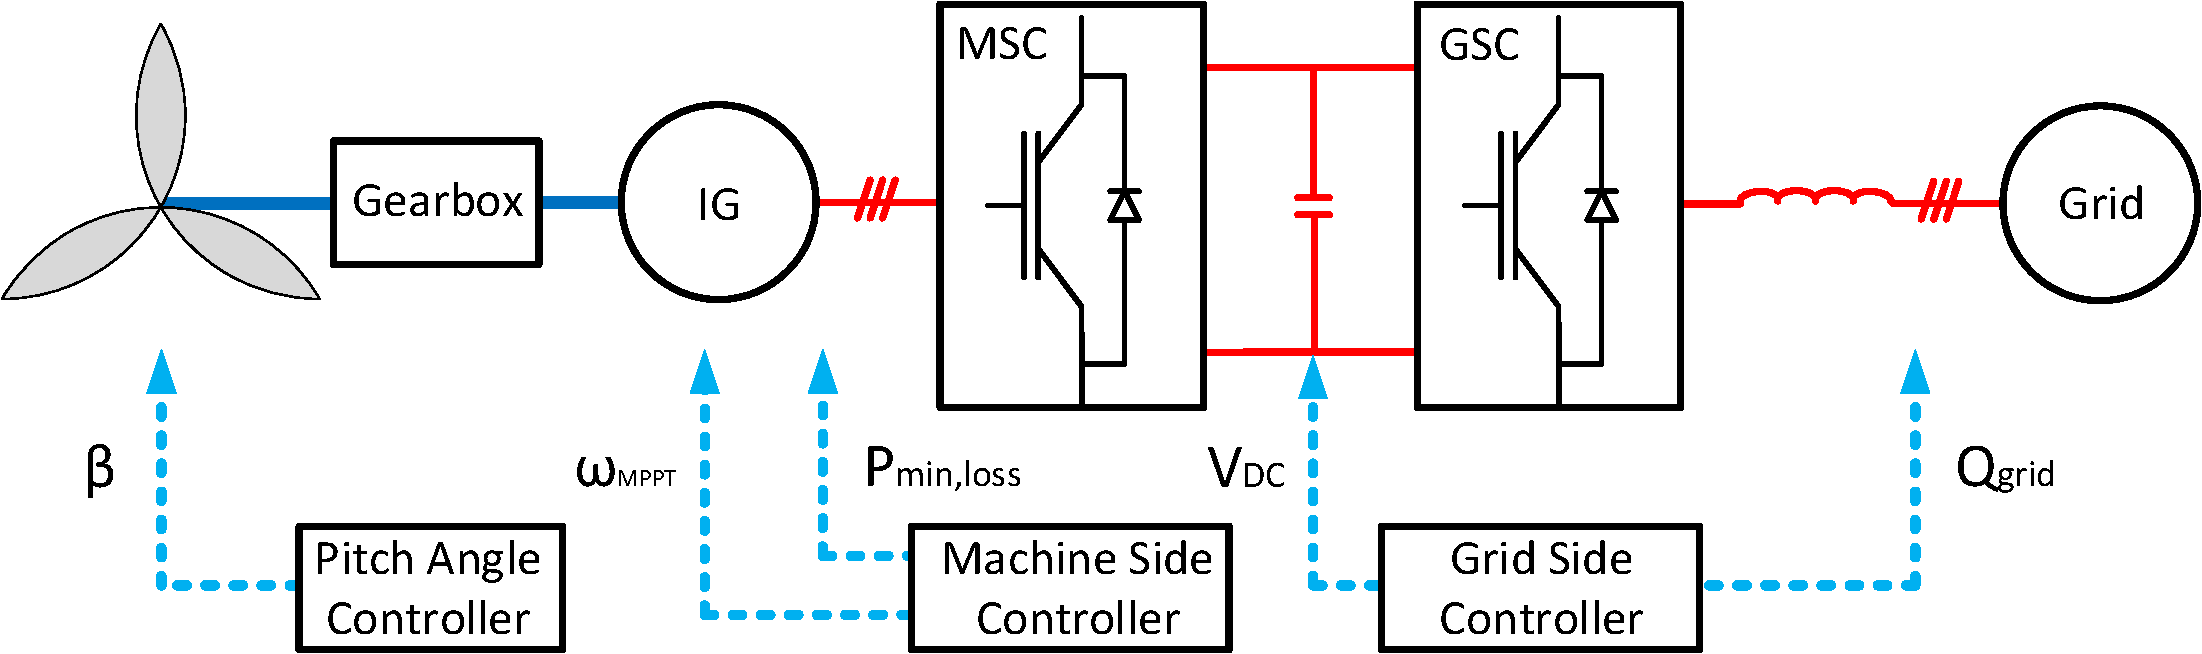
\includegraphics[width=0.9\linewidth]{windmodel2_2.pdf}
		\caption{Geared IG Wind Turbine}
		\label{varspeedpmsg_2}	
	\end{subfigure}
	\vspace{0.1em} % here you can insert horizontal or vertical space
	\begin{subfigure}{0.9\textwidth}
	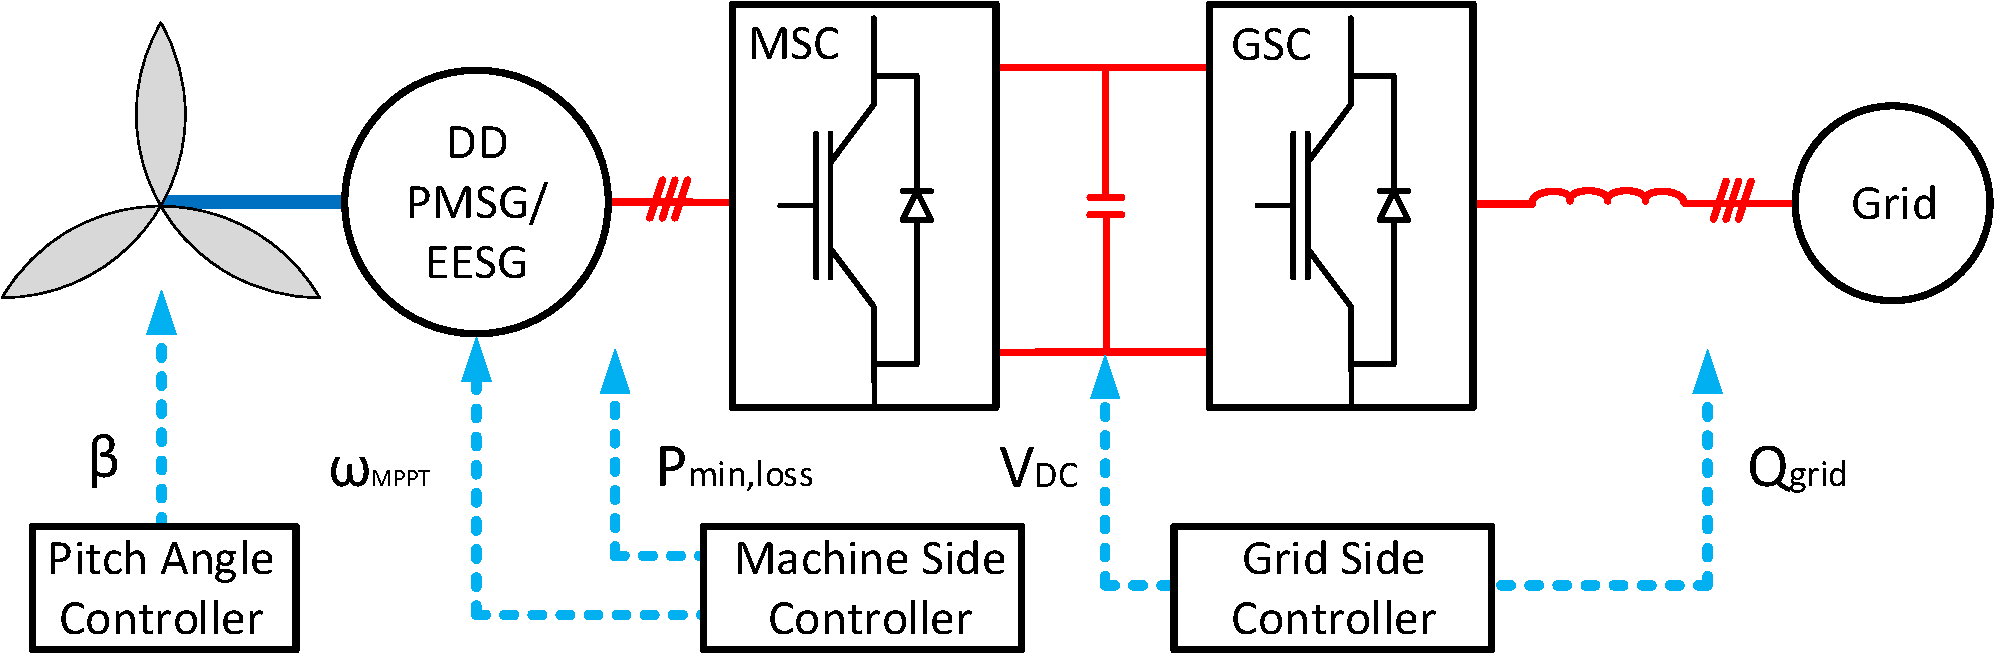
\includegraphics[width=0.9\linewidth]{windmodel2_3.pdf}
	\caption{Direct-Drive PMSG/EESG Wind Turbine}
	\label{varspeedpmsg_3}	
	\end{subfigure}
	\caption{Wind Turbine Topologies with Full-Scale Power Electronics}
\end{figure}
\subsection{Aerodynamic Model}
Aerodynamic model is the sub-model that captures power from the wind. The output of this block is the aerodynamic torque that rotates the turbine. However, the wind speed is not the only input. Turbine speed and pitch angle are also the inputs of the system since they affect the mechanical power that is captured from the wind.\par
The aerodynamic power of wind is given in Eq. (\ref{windpower}) where $\rho_{air}$ is air density in $kg/m^{3}$, $R$ is the blade radius in $m$ abd $v_{wind}$ is the wind speed in $m/s$. Note that this is the available power of the air that is striking the turbine swept area and it is not possible to extract that amount of energy. Otherwise, the air would be standstill behind the wind turbine \cite{Ackermann2005a}.
\begin{equation}
P_{wind}=0.5\rho_{air}\pi R^{2} v_{wind}^{3}
\label{windpower}
\end{equation}
The wind turbine captures a fraction of the available wind power that is denominated as power coefficient $C_{p}$. Therefore, turbine power captured from wind can be found with the Eq. (\ref{turbinepower}).
\begin{equation}
P_{tur}=C_{p}P_{wind}
\label{turbinepower}
\end{equation}
Power coefficient determines the amount of power to be captured from wind and it is a non-linear function of the tip speed ratio, $\lambda$ and pitch angle, $\beta$. Tip speed ratio is a parameter proportional with turbine speed. It can be defined as the ratio of the speed in the turbine tip to the wind speed as in the Eq. (\ref{tipspeed}). Power coefficient for a specific tip speed ratio and pitch angle can be found with the Eq. (\ref{cp}) and (\ref{lambdai}) where $c_{1}$ is 0.5176, $c_{2}$ is 116, $c_{3}$ is 0.4, $c_{4}$ is 5, $c_{5}$ is 21 and $c_{6}$ is 0.0068 \cite{Heier}.\par
\begin{equation}
\lambda=\frac{\omega_{tur}R}{v_{wind}}
\label{tipspeed}
\end{equation}
\begin{equation}
C_{p}(\lambda,\beta)=c_{1}(c_{2}/\lambda_{i}-c_{3}\beta-c_{4})e^{-c_{5}/\lambda{i}}+c_{6}\lambda
\label{cp}
\end{equation}
\begin{equation}
\frac{1}{\lambda_{i}}=\frac{1}{\lambda+0.08\beta}-\frac{0.035}{\beta^{3}+1} 
\label{lambdai}
\end{equation}
\begin{figure}[h!]
	\centering
	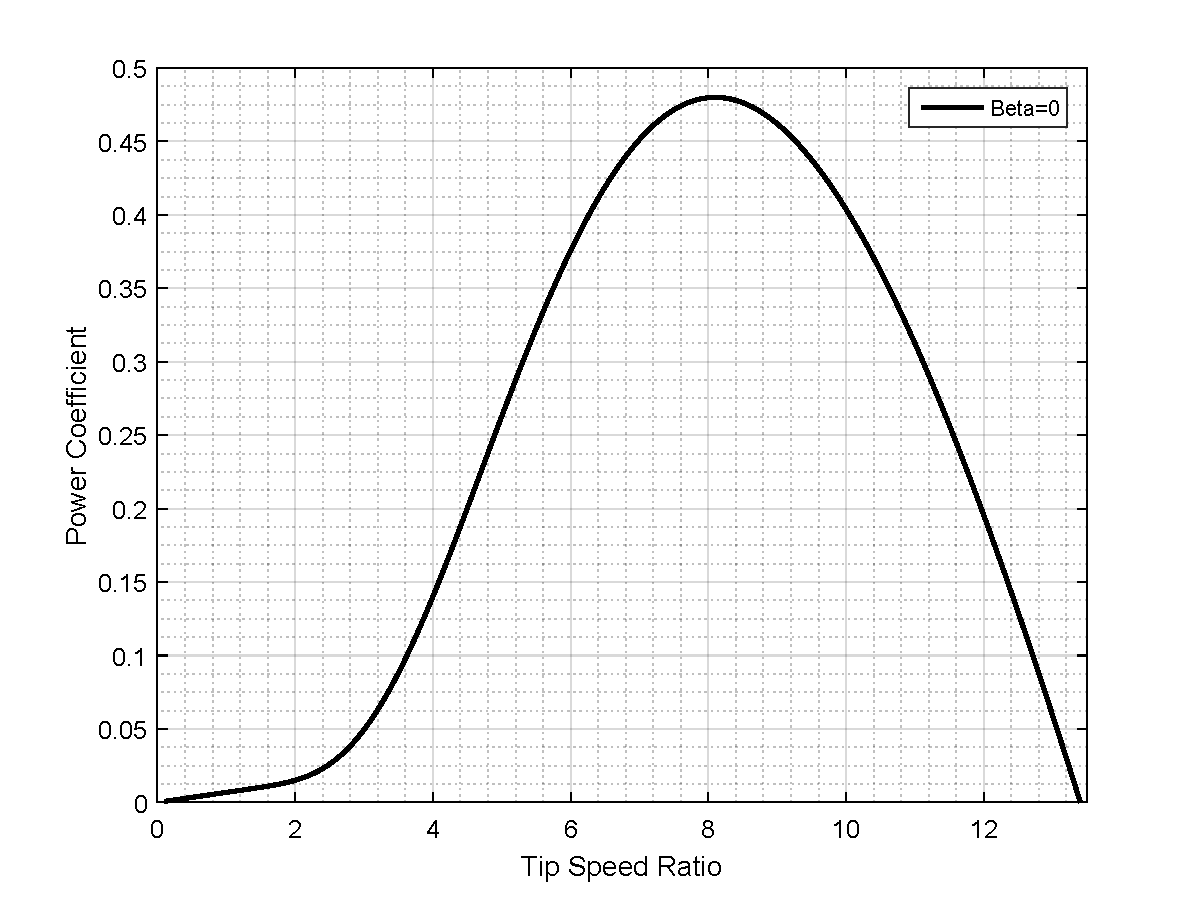
\includegraphics[width=.95\linewidth]{PowerCoefficient.pdf}
	\caption{Power Coefficient Variation with Tip Speed Ratio under Zero Pitch Angle}
	\label{variationofcp}
\end{figure} 
\par
Variation of power coefficient $C_{p}$ is given in Fig. \ref{variationofcp} for varying tip speed ratio. For the zero pitch angle, power coefficient has the maximum value of 0.48 for the tip speed ratio of 8.1. In order to ensure that the maximum of wind power is extracted, wind turbine should rotate a speed that gives the optimum tip speed ratio. This is ensured by the Maximum Power Point Tracking (MPPT) algorithms. 
\subsubsection{Maximum Power Point Tracking Algorithms}
In the literature, different methods are presented in order to operate in the Maximum Power Point. Perturb\&Obserb (P\&O) is the most common MPPT method in the literature \cite{Wang2004}, \cite{Barakati2009}. The methods simply creates a perturbation in the generator speed. The change in the generator speed creates also change in the active power output. If the power is increased with this perturbation, the generator speed is again perturbed in the same direction until a decrease in the active power is observed. This methods is the simplest method and does not require any calculation or wind speed measurement. However, the algorithm creates oscillations in the generator speed and active power. This method is also called as Hill-Climb Search (HCS) method in the literature.\par
Another MPPT algorithm is the wind speed measurement method \cite{Thriringer1993}, \cite{C.A.2013}. If the wind speed is estimated accurately, the optimal generator speed can be calculated. However, wind speed estimation is complicated and increases the cost. Another commonly used MPPT algorithm is the power-signal feedback (PSF) control \cite{C.A.2013},\cite{Wang2004}, \cite{Lu2002}. This method requires maximum power curve of the wind turbine based on the experimental results. A look-up table is constructed with obtained wind turbine speed and active output power values. However, using generator speed and active power measurements is the main drawback of this algorithm. Finally, there are numerous number of much complex MPPT algorithms based on fuzzy-logic \cite{Zeng2008} or neural-network \cite{Lin2011}. However, these MPPT algorithms are out of scope of this thesis. Therefore, optimal generator speed is provided in this study according to the wind speed. 
\subsubsection{Pitch Angle Control}
According to Eq. (\ref{windpower}), wind power increases with the cube of the wind speed. Hence, wind power increases dramatically for the high wind speeds. In order to decrease power, pitch angle i.e. blade angle is increased. Since the power coefficient, $C_{p}$ is a function of the pitch angle, $\beta$, wind power can be curtailed with increased blade angle. Variation of power coefficient for two different pitch angle is shown in Fig. \ref{cpwithtwopitchangle}. Increasing pitch angle by $1.176^{\circ}$ decreases power coefficient by 10\%.\par
\begin{figure}[h!]
	\centering
	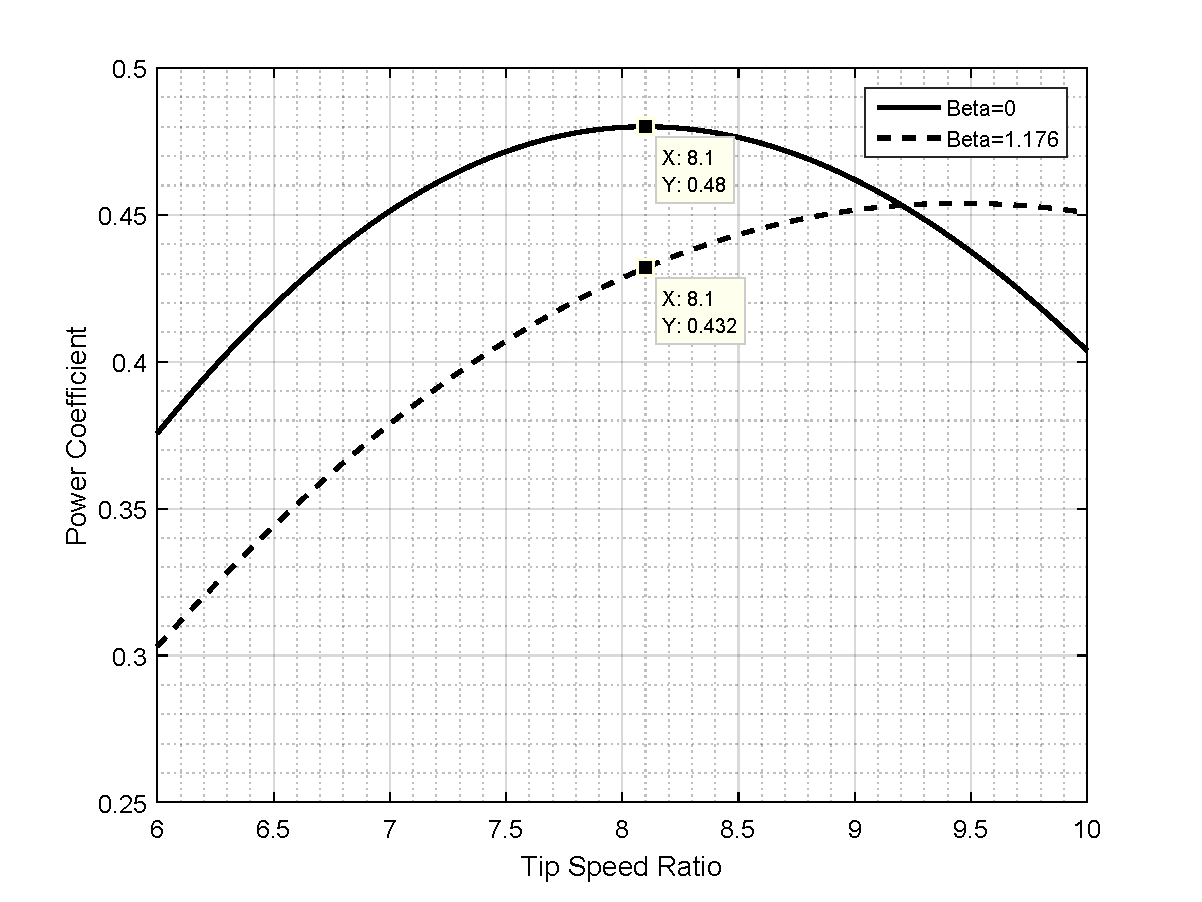
\includegraphics[width=.95\linewidth]{powercoefficient_with_varying_pitch.pdf}
	\caption{Power Coefficient Variation for Two Different Pitch Angle}
	\label{cpwithtwopitchangle}
\end{figure} 
As long as wind power is below the rated power, the wind turbine is operated in MPPT speed. This is ensured by obtaining optimal tip speed ratio. This means that for zero pitch angle, MPPT speed is increased linearly with wind speed. Before reaching rated power, MPPT speed might reach maximum generator speed. In this case, wind turbine reference speed will be the maximum generator speed. However, turbine speed cannot be decreased down to reference speed when the torque limit is reached. Hence, the pitch angle should be increased to regulate the turbine speed. Pitch angle controller is depicted in Fig. \ref{pitchcontroller}. Notice that the pitch angle is increased when the speed exceeds maximum generator speed. Otherwise, the pitch angle kept as zero.\par
\begin{figure}[h]
	\centering
	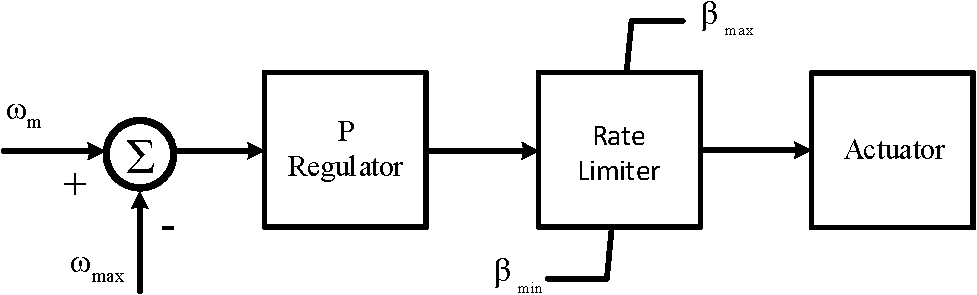
\includegraphics[width=.8\linewidth]{pitchcontroller2.pdf}
	\caption{Pitch Angle Control Diagram}
	\label{pitchcontroller}
\end{figure}
The responsibility of the pitch angle controller is the regulation of the blade angle but each blade in the wind turbine is a few tonnes. Therefore, the blade angle cannot be changed instantaneously and limited with rate limiter. The rate of change of pitch angle in this study is limited with $10^{\circ}/s$ \cite{Ackermann2005a}. Besides, the pitch angle controller takes action as soon as the maximum generator speed is exceeded. Therefore, wind turbine operation deviates from optimal tip speed ratio. This can also be observed from the variation of power coefficient, $C_{p}$ with the wind speed for the wind turbine GE 2.75-103 used in this study. Variation of the $C_{p}$ is shown in Fig. \ref{powercoefficientge}.
\begin{figure}[h!]
	\centering
	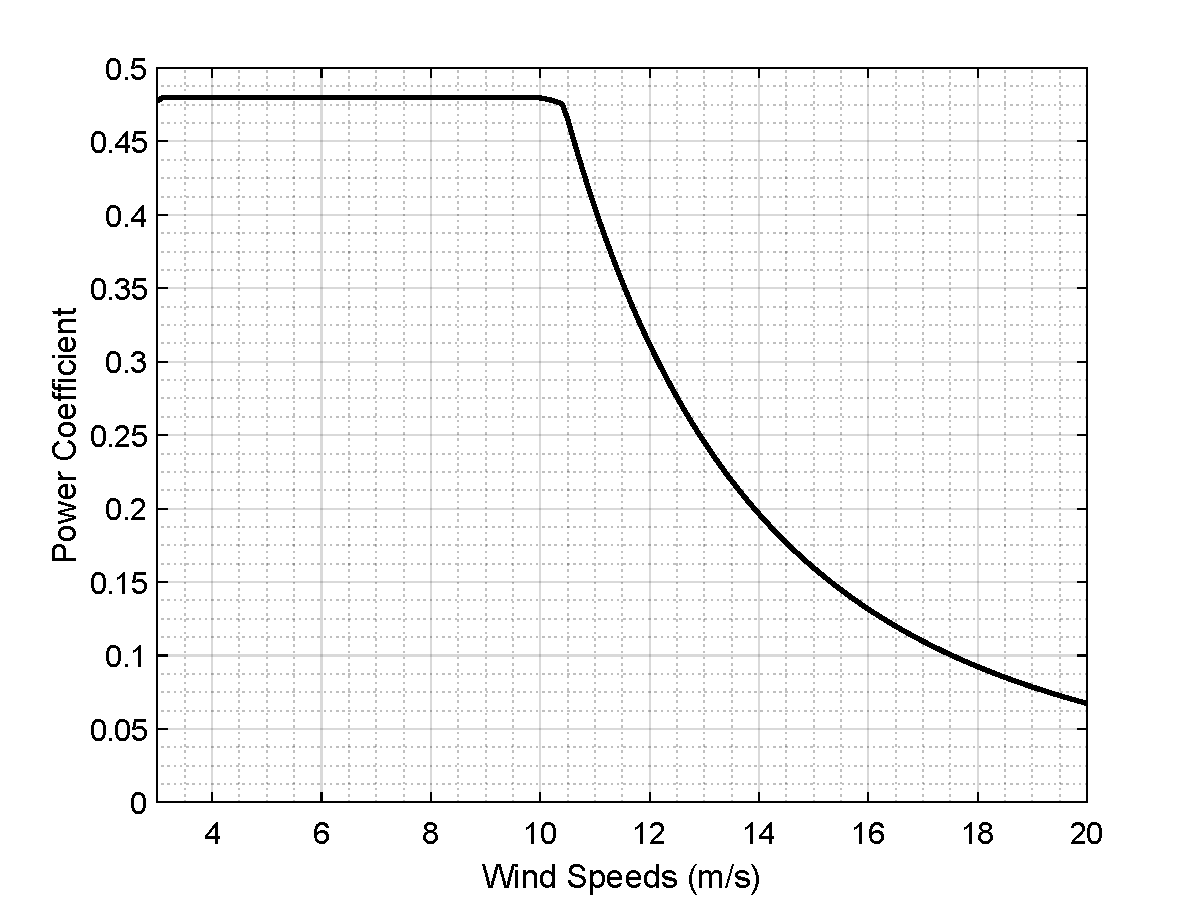
\includegraphics[width=.9\linewidth]{cp_wind.pdf}
	\caption{Power Coefficient Variation for GE 2.75-103}
	\label{powercoefficientge}
\end{figure}
\subsection{Gearbox}  
Variable speed PMSG wind turbines have a gearbox between turbine and generator except for direct-drive wind turbines. The gearbox increases angular speed and decreases the torque in the generator side. By decreasing the rated torque, generator size and cost can be reduced since the generator size is almost proportional to rated torque due to constant shear stress \cite{Polinder2013aa}. Moreover, turbine speed is increased to the allowable speed range of the generator which is generally much higher than that of wind turbines. Otherwise, generator should have high pole numbers. \par
A gearbox model is depicted in Fig. \ref{gearboxmodel}. They are mainly used for speed and torque conversion. It should be noted that the gearboxes are lossy systems. Therefore, the output torque of the gearbox would be lower than the ratio of input torque to gearbox conversion ratio. Direct-drive systems are based on the elimination of the gearbox systems by direct connection between turbine and generator in order to increase efficiency and reliability \cite{Chen2009b}. In this study, 3 stage (1 planetary / 1 helical) gearbox is modelled with \%97 efficiency \cite{UKONSAARI2016}. 
\begin{figure}[h!]
	\centering
	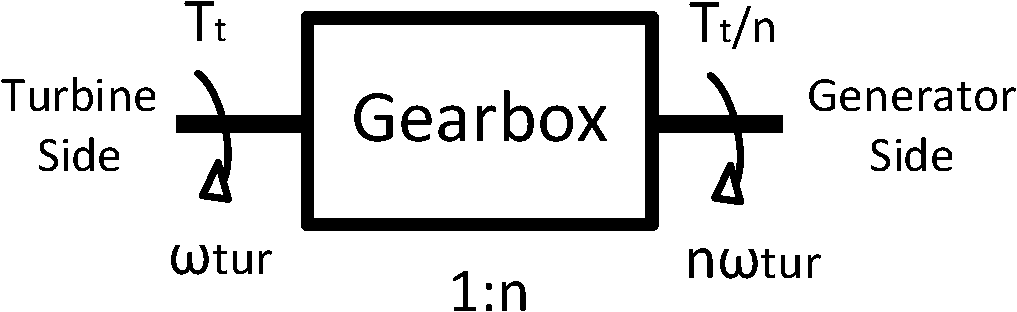
\includegraphics[width=.5\linewidth]{gearbox.pdf}
	\caption{Gearbox Modelling}
	\label{gearboxmodel}
\end{figure}
\subsection{Permanent Magnet Synchronous Generator}
\label{pmsgsection}
PMSGs and electrically excited generators can be employed with full-scale power electronics. However, PMSGs are generally preferred over electrically excited synchronous generators due to their high efficiency. The absence of electrical excitation on the rotor decreases losses. Besides, slip ring is not needed in the generator which also increases the reliability of the PMSG wind turbines. Dynamical equations of the salient pole PMSG are projected on a reference frame which rotates synchronously with magnet flux and given in Eq. (\ref{v1d}) and (\ref{v1q}) where $R_{1}$ is stator resistance in $\Omega$, $L_{sd}$ and $L_{sq}$ are d and q axis inductances in $H$, $i_{ad}$ and $i_{aq}$ are d and q axis currents in $A$, $\omega$ is the electrical angular frequency in $rad/s$, $\psi_{f}$ is magnet flux linkage in $Vs$ \cite{Ackermann2005a}. 
\begin{equation}
v_{1d}=R_{1} i_{ad}+L_{sd}\frac{di_{ad}}{dt}-L_{sq}\omega i_{sq}
\label{v1d}
\end{equation}
\begin{equation}
v_{1q}=R_{1} i_{aq}+L_{sq}\frac{di_{aq}}{dt}+L_{sd}\omega i_{sd}+\omega \psi_{f}
\label{v1q}
\end{equation}
Another important PMSG parameter is the power in dq frame. The power expression is given in Eq. (\ref{pmsgpower}). The electromechanical torque can be found by the relation between power and angular speed. The torque expression is also given in Eq. (\ref{pmsgtorque}) where p is the number of pole pair.
\begin{equation}
P_{elm}=\frac{3}{2}\omega i_{aq} (\psi_{f}+i_{ad}(L_{sq}-L_{sd}))
\label{pmsgpower}
\end{equation}
\begin{equation}
T_{e}=\frac{P_{elm}}{w_{m}}=\frac{P_{elm}}{w/p_{p}}=\frac{3}{2}p_{p} i_{aq} (\psi_{f}+i_{ad}(L_{sq}-L_{sd}))
\label{pmsgtorque}
\end{equation}

Given equations are defined for salient pole machines. If the clyndrical rotor machine is used, the torque equation reduces to the Equation \ref{pmsgtorque2}.
\begin{equation}
T_{e}=\frac{3}{2}p_{p} i_{aq} \psi_{f}
\label{pmsgtorque2}
\end{equation}
\subsection{Machine Side Converter}
Variable speed wind turbines that are equipped with the back-to-back converters are able to decouple grid frequency and the turbine speed. This gives wind turbine degree of freedom for the rotational speed. In this way, turbine is able to capture the maximum available power from wind. Machine Side Converter (MSC) i.e. Generator Side Converter is the converter that is connected between generator and DC-bus. The three phase generator output AC voltage is converted to DC voltage. Conversion from AC to DC can be achieved by three-leg full bridge converters. This converter can be equipped with uncontrolled, semi-controlled and fully-controlled switches. Fully-controlled switches such as MOSFET,IGBT are commonly used in the industry and gives two control parameters to the user. \par
Voltages and currents are generally transformed into synchronously rotating reference frame or also called dq frame. Since the frame is rotating in synchronous speed, three-phase phasors are transformed to DC quantities. Therefore, its control becomes easier \cite{Kazmierkowski2002}. Proportional-integral (PI) controllers are associated with the dq control structure due to their satisfactory behaviour interaction to DC variables \cite{Blaabjerg2006a}. Hence, the control in the back-to-back converter is achieved with PI controllers in the dq frame. \par
\begin{figure}[h!]
	\centering
	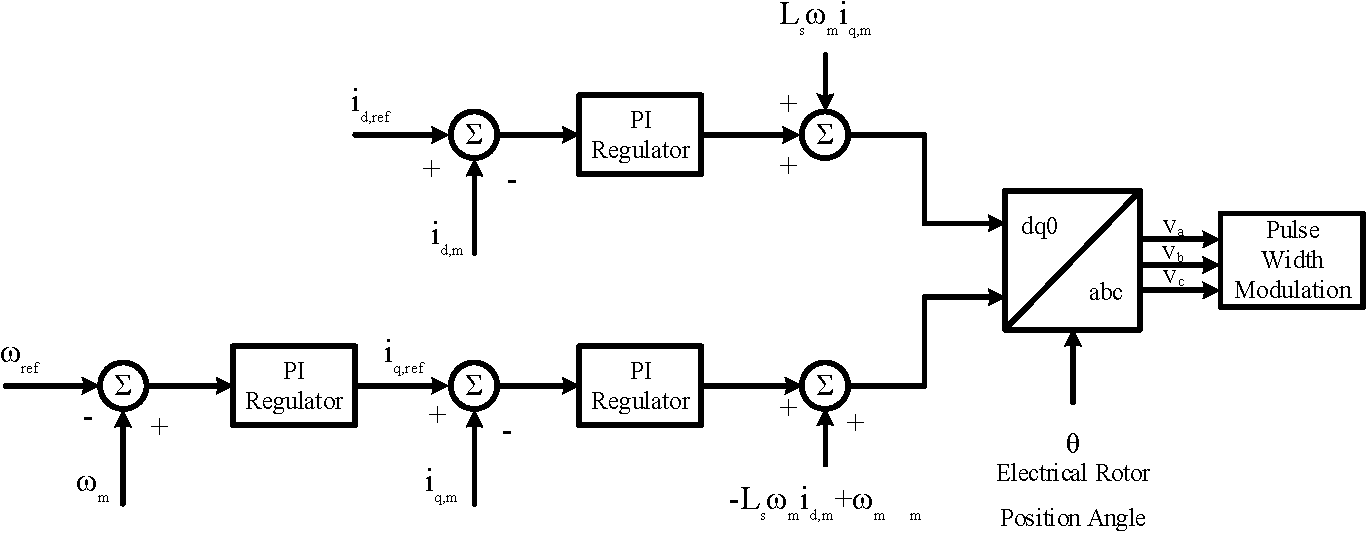
\includegraphics[width=.95\linewidth]{msc.pdf}
	\caption{Machine Side Controller Diagram}
	\label{msc}
\end{figure}
The control diagram of the MSC is depicted in Fig. \ref{msc} according to the study in \cite{Chinchilla2006}. In dq frame, it is possible to control two parameters. One of these parameters is the d-axis current that is set zero in order to decrease the stator copper losses. The other parameter is the q-axis current that is proportional to the electromagnetic torque as it can be observed in the Eq. (\ref{pmsgtorque2}). However, q-axis current or torque is controlled in order to regulate the turbine speed. Therefore, turbine speed is adjusted such that the turbine will capture maximum available power in the wind. 
\subsection{Grid Side Converter}
Grid Side Converter (GSC) or Line Side Converter (LSC) is the converter that is connected between DC-link capacitor and grid. GSC works as an inverter that injects current synchronous to grid. Currents and voltages are transformed into synchronously rotating frame that is aligned with the grid voltage. Therefore, d-axis current determines the amount of current which is in phase with the grid voltage meanwhile q-axis current determines amount of current that is out of phase with the grid voltage. In other words, injecting d-axis current injects active power to grid meantime q-axis current injects reactive power to grid.\par
The responsibility of the GSC is regulating DC voltage and the reactive power injected to the grid. The control diagram of the GSC is given in Fig. \ref{gsc}. As seen from the figure, DC-bus voltage is regulated by controlling the d axis current. If the DC-bus voltage increases above the reference value, d-axis current reference is increased. As a result, active power increases. Increased active power also decreases the DC-bus voltage level. Reference value of the q-axis current is set to zero in normal operation, consequently unity power factor. For Low Voltage Ride-Through studies, q-axis current is determined according to the reactive power value requirement. \cite{Orowska-Kowalska2014} \par
\begin{figure}[h!]
	\centering
	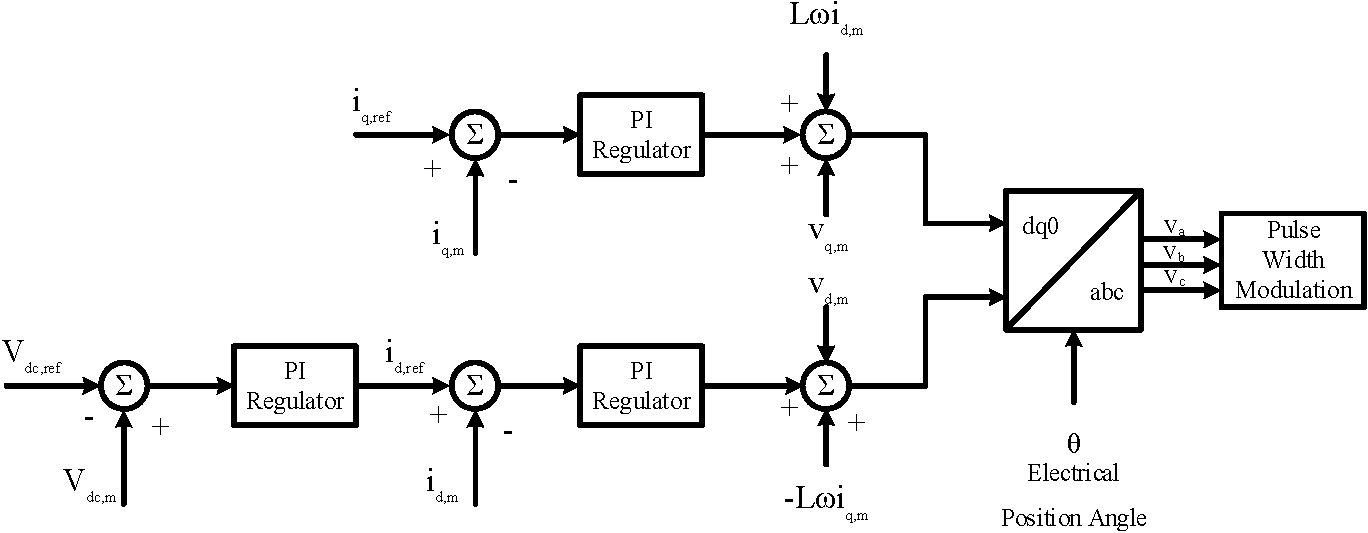
\includegraphics[width=.98\linewidth]{gsc.pdf}
	\caption{Grid Side Controller Diagram}
	\label{gsc}
\end{figure}
GSC is connected to grid through a filter. Therefore, the output voltage of the converter is not equal to the that of grid. The relation between converter voltage, grid voltage and current is derived through Eq. (\ref{crossilk}) to (\ref{crosscomp2}) where $v_{c}$ is the converter voltage, $v_{g}$ is the grid voltage and  $i_{g}$ is the grid current measured in the grid side. As it is observed in Eq (\ref{crosscomp1}) and (\ref{crosscomp2}), converter side voltage includes same axis grid voltage and a term proportional to cross axis current which is called cross-coupled term. Therefore, the outputs of the inner PI regulators are compensated and forwarded to Pulse Width Modulation after transformation to three-phase voltages.
\begin{equation}
\overline{v_{c}}=v_{dc}+jv_{qc}
\label{crossilk}
\end{equation}
\begin{equation}
\overline{v_{g}}=v_{dg}+jv_{qg}
\end{equation}
\begin{equation}
\overline{i_{g}}=i_{dg}+ji_{qg}
\end{equation}
\begin{equation}
\overline{v_{c}}=\overline{v_{g}}+\overline{i_{g}}j\omega L
\end{equation}
\begin{equation}
v_{dc}+jv_{qc}=v_{dg}+jv_{qg}+j\omega L (i_{dg}+ji_{qg})
\end{equation}
\begin{equation}
v_{dc}=v_{dg}-\omega L i_{qg}
\label{crosscomp1}
\end{equation}
\begin{equation}
v_{qc}=v_{qg}+\omega L i_{dg}
\label{crosscomp2}
\end{equation}
The PI regulators of the wind turbine model is tuned with trial error method. In this study, the modelled wind turbine is connected to grid with an L filter even though the actual turbine is connected to grid with an LCL filter. However, the actual system would operate better than the modelled case since the the LCL filter has superior performance than L filters \cite{Brantsater2015}. Nonetheless, L filter has provided sufficient performance for the successful operation of the wind turbine in this study regardless from the power quality standards in the output current. The active power of the wind turbine under varying wind speed is given in the Fig. \ref{powerdata}. \par
\begin{figure}[h!]
	\centering
	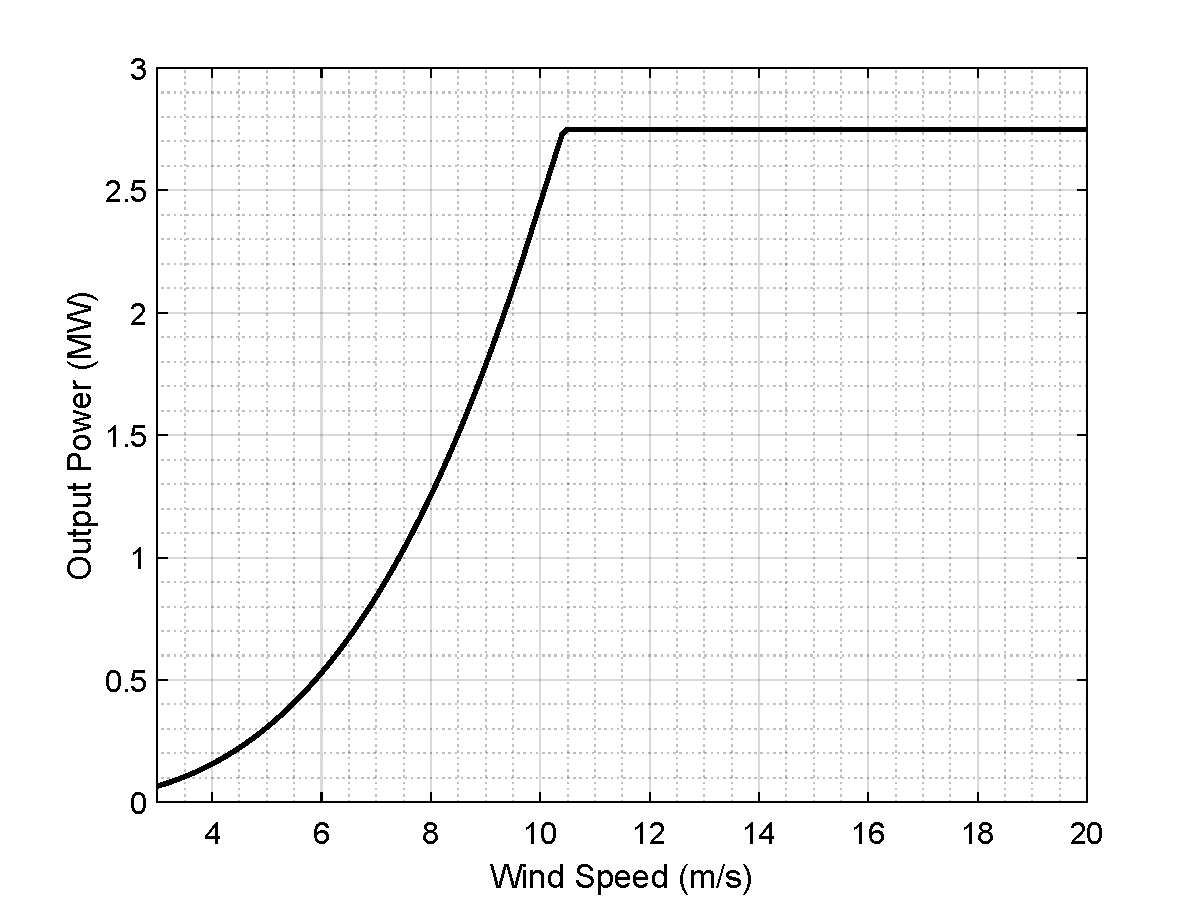
\includegraphics[width=.9\linewidth]{powerdata.pdf}
	\caption{Variation of the Active Power of the Wind Turbine}
	\label{powerdata}
\end{figure}
\section{Synthetic Inertia Implementation}
As explained Section \ref{swing}, synchronous generators change their speed according to the balance between input mechanical and electromechanical powers. Furthermore, if the frequency changes, the electromechanical power of the generators also change. Nonetheless, the renewable energy systems which are connected to grid with a power electronics interface are unresponsive to the deviations in the grid frequency.\par
The definition of the synthetic inertia is the controlled contribution of electrical torque that is proportional to RoCoF in the unit connection terminal \cite{Eriksson2017}. Synthetic inertia (also called as 'virtual inertia') is the method that emulates the synchronous generator in the renewable energy systems. In this method, the active power output of the wind turbines are adjusted according to the Eq. (\ref{synthetic}) where $H_{syn}$ is the synthetic inertia constant in seconds and $\omega_{t}$ is the terminal angular frequency in pu. The increase in the active power is proportional to RoCoF as well as the emulated inertia constant. The emulated inertia constant can be different from the inertia constant of the renewable energy system. For instance, the solar PV systems does not have inertia. Even in these systems, an inertia constant can be emulated as long as the system includes stored energy. In the wind turbines, the additional energy can be yielded from the kinetic energy in the turbine inertia. For solar PV systems, energy storage systems or the store energy in the DC-link capacitor can be utilized.\par
\begin{equation}
\Delta P_{e}=-2H_{syn}\frac{d\omega_{t}}{dt}\omega_{t}
\label{synthetic}
\end{equation}
In order to implement synthetic inertia in the system, a relation between frequency and active power of the wind turbine should be constructed. Wind turbine in this study is variable speed wind turbine with full scale power electronics. The speed of the turbine is controlled by MSC such that active power is adjusted. Inertial support modification is depicted in Fig. \ref{modifiedmsc}. The new value of the active power is determined according to the swing equation. However, the wind turbine in this study is operated with a reference speed rather than a reference power. Therefore, the assigned power value should be used in order to yield the q-axis current reference value. Reference q-axis current is derived between the Eq. (\ref{inertialsupport1}) to Eq. (\ref{inertialsupport4}).\par
\begin{figure}[h!]
	\centering
	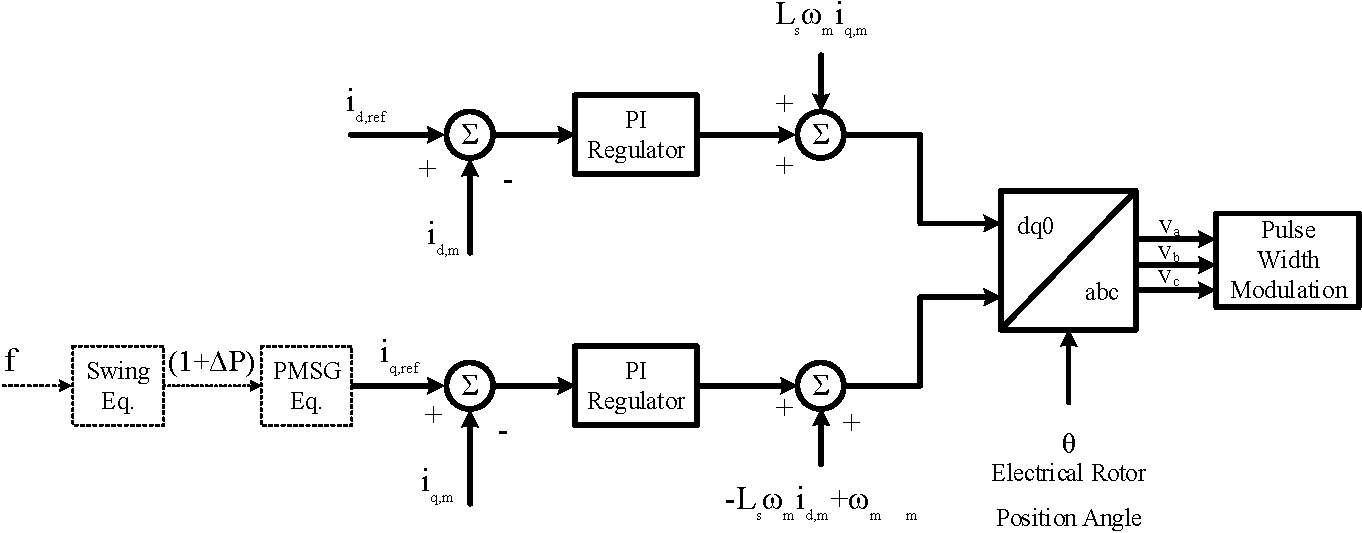
\includegraphics[width=.98\linewidth]{msc_modified.pdf}
	\caption{Modified MSC for Inertial Support}
	\label{modifiedmsc}
\end{figure}
\begin{equation}
P_{new}=(1+\Delta P) P_{pre}
\label{inertialsupport1}
\end{equation}
\begin{equation}
T_{new} \omega_{m}=(1+\Delta P) T_{pre} \omega_{pre}
\label{inertialsupport2}
\end{equation}
\begin{equation}
\frac{3}{2} p_{p} \psi_{f} i_{q,new} \omega_{m}=(1+\Delta P) \frac{3}{2} p_{p} \psi_{f} i_{q,pre} \omega_{pre}
\label{inertialsupport3}
\end{equation}
\begin{equation}
 i_{q,ref}=i_{q,new}=(1+\Delta P) \frac{i_{q,pre} \omega_{pre}}{ \omega_{m}} 
\label{inertialsupport4}
\end{equation}
\subsection{Synthetic Inertia Activation Schemes}
Another issue about inertial support is the time instant to trigger synthetic inertia. In the literature, continuous operation, under-frequency trigger and maximum-frequency gradient are discussed \cite{Gonzalez-longatt2015}. It is obvious that continuous operation would create oscillations in active power output due to the continuous deviations in grid frequency. This is an unrealistic operation and is used for comparison purposes.\par
Second activation method is the under-frequency trigger which is the activation when the frequency decreases below a threshold value. It can be used for capturing the time instant for the inertial support. However, power grid might be in a stable point even if the frequency is 49.8Hz. Therefore, this method would be unsuccessful depending on the disturbance event. \par 
Third activation scheme is the maximum-frequency gradient trigger. It uses a controller that is very similar to RoCoF relays and tracks the frequency gradient. Once the frequency gradient is below a threshold value, the synthetic inertia is activated. Since the severity of frequency disturbance event is related to the RoCoF, this activation scheme is the most remarkable scheme \cite{Gonzalez-longatt2015}. \par The activation of the inertial support by only frequency-gradient (RoCoF) might be misleading. For instance, a negative RoCoF value when the frequency is above the nominal value is not a frequency disturbance. Therefore, the inertial support should not be activated unless the frequency is below a threshold. Thus, in this study, maximum-frequency gradient is used in coordination with the under-frequency trigger. \par 
Grid RoCoF changes in the grid according to the disturbance level as well as the grid inertia. According to the disturbances in the Continental Europe System within the last 15 years, RoCoFs in the range between 0.1Hz/s and 1Hz/s are observed \cite{ENTSO-E2016}.Therefore in this study, 0.1Hz/s of RoCoF threshold with a frequency dead-band of 10mHz is selected. In this way, a negative RoCoF above 49.99Hz is not captured as events as long as it does not decrease below the under frequency threshold.
\subsection{Source of the Inertial Support}
The renewable energy systems cannot determine the amount of power in contrast the conventional systems. A thermal power plant, for instance, adjusts its power output as desired. However, the source of power in renewable energy is intermittent due to nature of the power source. This is why a spare energy is required in order to change the power output.\par
The stored energy in a wind turbine exists in the generator and turbine inertia. Therefore, the drive train of the wind turbine is important for the stored energy in the turbine. Different drive train concepts are compared in Table \ref{gencompare} according to the typical generator data presented in \cite{Seman2011}. According to the typical generator data and typical gearbox ratios, the stored energy with the High Speed Full Converter (HSFC) is calculated as 16.2MJ meanwhile DFIG concept stored 15.7MJ. However, the Direct-Drive concept stores 13.6MJ energy. Even though the stored energies close to each other, it is observed that the higher speed generator concepts store more than that of lower speed concepts. Notice that the wind turbine studied in thesis is a 3 stage HSFC wind turbine which store the highest energy compared to the other drive trains in the same power class.
% Please add the following required packages to your document preamble:
% \usepackage{graphicx}
\begin{table}[h!]
	\centering
	\resizebox{\textwidth}{!}{%
		\begin{tabular}{|c|c|c|c|c|}
			\hline
			\textbf{\begin{tabular}[c]{@{}c@{}}Drive\\   Train Concept\end{tabular}}       & \begin{tabular}[c]{@{}c@{}}Doubly-Fed \\ 3 Stage Gear\end{tabular} & \begin{tabular}[c]{@{}c@{}}Low Speed\\ Full Converter \\ (LSFC)\\   Direct Drive\end{tabular} & \begin{tabular}[c]{@{}c@{}}Medium Speed\\ Full Converter\\   (MSFC) \\ 2 Stage Gear\end{tabular} & \begin{tabular}[c]{@{}c@{}}High Speed\\ Full Converter\\  (HSFC)\\ 3 Stage Gear\end{tabular} \\ \hline
			\textbf{Generator Type}                                                        & DFIG                                                               & PMSG                                                                                          & PMSG                                                                                             & PMSG                                                                                         \\ \hline
			\textbf{\begin{tabular}[c]{@{}c@{}}Generator\\ Inertia \\ (kgm2)\end{tabular}} & 250                                                                & 40500                                                                                         & 510                                                                                              & 115                                                                                          \\ \hline
			\textbf{\begin{tabular}[c]{@{}c@{}}Generator Speed\\   (rpm)\end{tabular}}     & 1200                                                               & 14                                                                                            & 400                                                                                              & 1600                                                                                         \\ \hline
			\textbf{\begin{tabular}[c]{@{}c@{}}Gearbox\\   Ratio\end{tabular}}             & 85                                                                 & -                                                                                             & 28                                                                                               & 110                                                                                          \\ \hline
			\textbf{\begin{tabular}[c]{@{}c@{}}Blade\\   Inertia\\ (kgm2)\end{tabular}}    & 12600000                                                           & 12600000                                                                                      & 12600000                                                                                         & 12600000                                                                                     \\ \hline
			\textbf{\begin{tabular}[c]{@{}c@{}}Stored\\   Energy (MJ)\end{tabular}}        & 15.7                                                               & 13.6                                                                                          & 14.5                                                                                             & 16.2                                                                                         \\ \hline
		\end{tabular}%
	}
	\caption{Stored Energy Comparison for Different Drive Train Concepts}
	\label{gencompare}
\end{table}
\begin{equation}
E_{electrostatic}=\frac{1}{2} C_{DC}V_{DC}^{2}
\label{electrostatic}
\end{equation}
Energy stored in DC bus capacitor is the only stored energy in PV systems. The amount of energy is given in Eq. (\ref{electrostatic}) and negligible for inertial support studies. In the wind energy systems, there exists significant amount of kinetic energy (above 10MJ) in wind turbine generator and blades in addition to electrostatic energy. The kinetic energy expression is given in Eq. (\ref{kineticenergy}). It should be noted that $J_{total}$ is the equivalent inertia in the generator side as given in Eq. (\ref{totalinertia}),$n$ is the gearbox conversion ratio and $\omega_{m}$ is the speed of the generator.
\begin{equation}
J_{total}=\frac{J_{tur}}{n^{2}} + J_{gen}
\label{totalinertia}
\end{equation}
\begin{equation}
E_{kinetic}=\frac{1}{2} J_{total}\omega_{m}^{2}
\label{kineticenergy}
\end{equation}
Notice that the amount of kinetic energy is dependent on the generator speed. Therefore, the stored energy in wind turbine change according to the generator speed. Moreover, it can also be concluded that the energy is dependent on the wind speed. However, the generator speed is kept constant if the wind speed increases above the rated wind speed. \par
To illustrate the situation better, the electrostatic energy stored in DC bus and kinetic energy in turbine equivalent inertia are compared for GE2.75-103 wind turbine. The wind turbine has a DC bus capacitance of $27mF$ and $1200V$ DC link voltage. The corresponding electrostatic energy is calculated in Eq. (\ref{electrostatic2}). The generator speed of the corresponding generator is between $550rpm$ and $1735rpm$. The total turbine inertia is $1058.2 kgm^2$ in the generator side. The minimum and maximum kinetic energy values are calculated in Eq. (\ref{kineticenergymin}) and (\ref{kineticenergymax}). \par
\begin{equation}
E_{DC-Link}=\frac{1}{2} 27 (10^{-3}) 1200^{2}=19.44kJ
\label{electrostatic2}
\end{equation}
\begin{equation}
E_{kinetic,min}=\frac{1}{2} (1058.2) 57.6^{2}=1755.17kJ
\label{kineticenergymin}
\end{equation}
\begin{equation}
E_{kinetic,max}=\frac{1}{2} (1058.2) 181.7^{2}=17466.02kJ
\label{kineticenergymax}
\end{equation}
It is obvious that the stored kinetic energy in the wind turbine is 90 times of the energy stored in DC bus capacitor even in the minimum generator speed. Therefore, utilization of the kinetic energy for inertial support studies is more efficient than using the stored energy in the capacitor. \par
\begin{table}[h]
	\centering
	\begin{tabular}{ccc}
		\hline
		Parameters                                                           & Minimum & Maximum \\ \hline
		\begin{tabular}[c]{@{}c@{}}Generator Speed\\ (rad/s)\end{tabular}    & 57.6    & 181.7   \\
		\begin{tabular}[c]{@{}c@{}}Stored Kinetic Energy\\ (kJ)\end{tabular} & 1755    & 17466   \\
		\begin{tabular}[c]{@{}c@{}}Inertia Constant\\ (s)\end{tabular}       & 0.58    & 5.75    \\ \hline
	\end{tabular}
	\caption{Dynamic Parameters of the Wind Turbine}
	\label{windpar}
\end{table}
Dynamical parameters of the wind turbine are listed in the Table \ref{windpar}. The stored energy in the turbine equivalent inertia varies with the square of the generator speed. Therefore, the minimum stored energy is one tenth of the maximum case. As a result of this, the inertia constant of the wind turbine is dependent on the wind speed and varies between 0.58s and 5.75s. Notice that the inertia constants to be emulated by wind turbine in this thesis are not restricted to these inertia constant. Wind turbines can emulate higher inertia constants as long as they can increase the output power to desired levels.
\section{Conclusion}
In this chapter, the detailed modelling for PMSG wind turbine is presented. The MSC which is responsible for adjusting the turbine speed for MPPT operation is modified such that the wind turbine provides inertial support. The additional active power is obtained with the kinetic energy extraction from the turbine inertia. \par
The requirement of the inertial support provision is the back-to-back converter that enables the active power and speed control. Therefore, the method described in this chapter is not specific to PMSG wind turbines but the ones with full-scale power electronics. 

\bibliographystyle{ieeetr} 
\bibliography{library} 

%
% References in Bibtex format goes into below indicated file with .bib extension
%\bibliography{thesis_references}
% You can use full name of authors, however most likely some of the Bibtex entries you will find, will use abbreviated first names
% If you don't want to correct each of them by hand, you can use abbreviated style for all of the references

%\bibliographystyle{abbrv}

% if you have more that one appendix, then use \appendices, otherwise use 
\appendix
\chapter{Ek A }
\label{chp:appendixA}

\section{Örnek Kısım}
Kısım içine yazılacaklar...


\end{document}
